%%%%%%%%%%%%%%%%%%%%%%%%%%%%%%%%%%%%%%%%%%%%%%%%%%%%%%%%%%%%%%%%%%%%
%% I, the copyright holder of this work, release this work into the
%% public domain. This applies worldwide. In some countries this may
%% not be legally possible; if so: I grant anyone the right to use
%% this work for any purpose, without any conditions, unless such
%% conditions are required by law.
%%%%%%%%%%%%%%%%%%%%%%%%%%%%%%%%%%%%%%%%%%%%%%%%%%%%%%%%%%%%%%%%%%%%

\documentclass{beamer}
\usetheme[faculty=wi]{fibeamer}
\usepackage[utf8]{inputenc}
\usepackage[
  main=french,
  french
]{babel}

\title{Language C}
\subtitle{Université de Lorraine - Télécom Nancy}
\author{Omar CHIDA}

\usepackage{ragged2e}  % `\justifying` text
\usepackage{booktabs}  % Tables
\usepackage{tabularx}
\usepackage{tikz}      % Diagrams
\usetikzlibrary{calc, shapes, backgrounds}
\usepackage{amsmath, amssymb}
\usepackage{url}       % `\url`s
\usepackage{listings}  % Code listings
\usepackage{xcolor}
\usetikzlibrary{backgrounds,positioning,matrix,arrows,arrows.meta}
\usepackage{drawstack}

\frenchspacing
\begin{document}
  \frame[c]{\maketitle}

  \AtBeginSection[]{% Print an outline at the beginning of sections
    \begin{frame}<beamer>
      \frametitle{Chapitre \thesection : \secname}
      \tableofcontents[currentsection,currentsubsection,subsectionstyle=show/show/hide]
    \end{frame}}

	\AtBeginSubsection[] {
		\begin{frame}<beamer>
			\frametitle{Chapitre \thesection : \secname}
			\framesubtitle{Section \thesubsection : \subsecname}
			\tableofcontents[currentsection,currentsubsection,sectionstyle=show/hide,subsectionstyle=show/shaded/hide]  
		\end{frame}
	}

  \begin{darkframes}
  	\section{Introduction}

\subsection{Remerciement}
\begin{frame}{Remerciement}
	\framesubtitle{Sans eux, ce ne sera pas possible}
	\begin{itemize}
		\item Un grand merci à M.Bouthier et M.Oster de m'avoir fait confiance et de m'avoir permis de préparer ces conférences.
		\item Un grand merci à Mme.Collin pour m'aider avec les problèmes administratifs et pour avoir accéléré la mise en place de cette leçon
		\item Merci à l'Université de Lorraine et à Télécom Nancy de m'avoir permis de préparer ces tutorats.
	\end{itemize}
\end{frame}

\subsection{À propos de moi}
\begin{frame}{À propos de moi}
	\framesubtitle{Savoir plus: \url{omarito.com}}
	\begin{columns}[T] % align columns
		\begin{column}{.71\textwidth}
			\begin{itemize}
				\item Education:
				\begin{itemize}
					\item Bac Mathématiques
					\item Licence Informatique
				\end{itemize}
				\item Premier ligne de code à l'âge de 14 ans.
				\item Grand fan de C++: 6 ans de C/C++.
				\item De nombreux projets dont un moteur de rendu, une application mobile entre autres codée en C/C++.
			\end{itemize}
		\end{column}%
		\hfill%
		\begin{column}{.25\textwidth}
			\begin{tikzpicture}[overlay,remember picture]
				\node[anchor=south east,xshift=-20pt,yshift=70pt]
				at (current page.south east) {
					
\includegraphics[width=35mm]{resources/omarito}
				};
			\end{tikzpicture}%
		\end{column}%
	\end{columns}
\end{frame}
\subsection{Organisation}
\begin{frame}{Organisation}
	\framesubtitle{Comment ça va se passer?}%
	\begin{itemize}
		\item Cours, exercices, solutions et projets seront sur \href{https://github.com/Darhal/TeachingC}{Github}.
		\item Serveur \href{https://discord.gg/y9nYQ5A5Fz}{Discord} dédié pour les questions, aide et autre.
		\item TD, TP et Projets seront en présentiel.
		\item N'hésitez pas à m'interrompre à tout moment pour poser des questions.
	\end{itemize}
\end{frame}
\subsection{L'objectif du Tutorat}

\begin{frame}{L'objectif du Tutorat}
	\begin{itemize}
		\item Vous familiariser avec la Langage C.
		\item Connaître les bonnes pratiques de programmation en C.
		\item Réussir les examens mais ça va aussi plus loin que ça.
		\item Compréhension approfondie des pointeurs et de la gestion de la mémoire en C.
		\item Bien comprendre l'outillage (Compilateur, Débogueur, autre).
	\end{itemize}
\end{frame}

\begin{frame}{L'objectif du Tutorat}
	\framesubtitle{Ce que vous pourrez faire à la fin}%
	\begin{columns}[T] % align columns
		\begin{column}{.48\textwidth}
			\begin{tikzpicture}[overlay,remember picture]
				\node[anchor=south west,xshift=10pt,yshift=70pt]
				at (current page.south west) {
					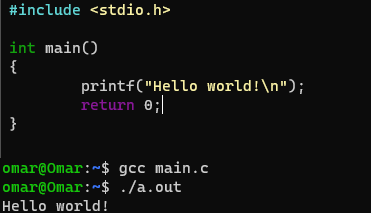
\includegraphics[scale=0.5]{resources/begin}
				};
			\end{tikzpicture}%
		\end{column}%
		%\hfill%
		\begin{column}{.065\textwidth}
			\begin{tikzpicture}[overlay,remember picture]
				\node[anchor=south west,xshift=160pt,yshift=110pt]
				at (current page.south west) {
					$\implies$
				};
			\end{tikzpicture}%
		\end{column}%
		\begin{column}{.48\textwidth}
			\begin{tikzpicture}[overlay,remember picture]
				\node[anchor=south east,xshift=-10pt,yshift=55pt]
				at (current page.south east) {
					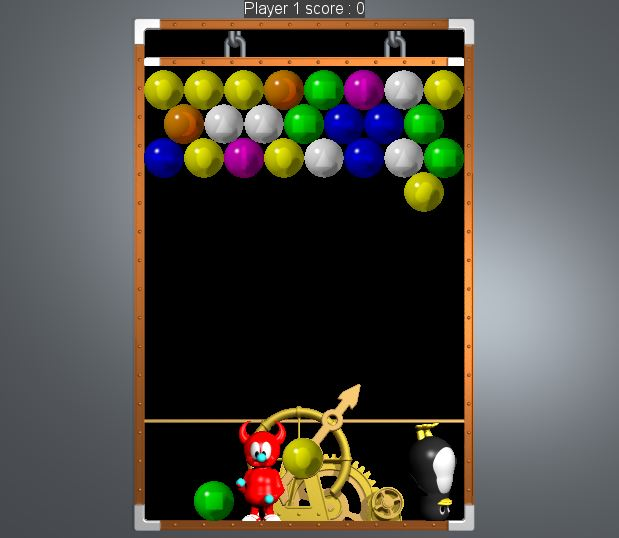
\includegraphics[scale=0.32]{resources/end}
				};
			\end{tikzpicture}%
		\end{column}%
	\end{columns}
\end{frame}

\begin{frame}{L'objectif du Tutorat}
	\framesubtitle{Ce que nous allons faire ensemble}%
	\begin{itemize}
		\item Plein d'exercices (même style que les TD).
		\begin{itemize}
			\item Exercices liés aux structures de données.
			\item Savoir des techniques intelligentes pour avoir un code C plus rapide (de l'optimisation)
		\end{itemize}
		\item Il y aura un gros projet à la fin.
		\begin{itemize}
			\item Un jeu vidéo du style (Puzzle Bobble ou Mario).
			\item Jeu sur le terminal (style Snake).
			\item Émulateur de processeur ARM.
			\item Quelque chose de plus simple que ça? (n'hésitez pas à déposer vos idées).
		\end{itemize}
	\end{itemize}
\end{frame}

\subsection{À propos de C}
\begin{frame}{À propos de C}
	\framesubtitle{Un peu de connaissances générales}%
	% dennis_ritchie
	\begin{columns}[T] % align columns
		\begin{column}{.76\textwidth}
			\begin{itemize}
				\item Langage conçu par Dennis Ritchie et développé par lui et Bell labs.
				\item Sortie en 1972 (il y a 49 ans).
				\item Utilisé dans le projet Unix développé par Dennis Ritchie et Ken Thompson entre autres.
				\item A vu une évolution relativement petite.
				\begin{itemize}
					\item K\&R C, ANSI C, C99, C11, C17, C2x.
				\end{itemize}
				\item Aujourd'hui, C est considéré comme un langage de bas niveau.
			\end{itemize}
		\end{column}%
		\hfill%
		\begin{column}{.20\textwidth}
			\begin{tikzpicture}[overlay,remember picture]
				\node[anchor=south east,xshift=-10pt,yshift=50pt]
				at (current page.south east) {
					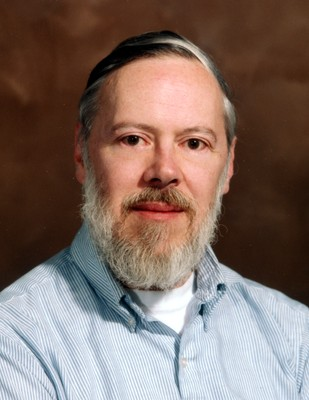
\includegraphics[width=30mm]{resources/dennis_ritchie}
				};
			\end{tikzpicture}%
		\end{column}%
	\end{columns}
\end{frame}

\subsection{Motivation : Pouquoi apprendre le C en 2021?}
\begin{frame}{Motivation : Pouquoi apprendre le C en 2021?}
	\framesubtitle{C c'est cool !}%
	\begin{itemize}
		\item C est toujours pertinent et utile aujourd'hui pour beaucoup de choses.
		\item Développement des noyaux (Kernel) et des systèmes d'exploitation
		\item Systèmes embarqués (véhicules, caméras, satellites, IoT, ...)
		\item Développement de pilotes de périphériques (Device Drivers)
		\item Bibliothèques et frameworks hautes performances (Numpy, ...)
		\item Compilateurs et interprètes de nombreuses langues populaires (Java, Python, ...).
		\item Moteurs de rendu et jeux vidéo.
		\item Bref... partout où la performance est essentielle.
	\end{itemize}
\end{frame}
	\section{Compilation}
\begin{frame}{Compilation}
	\begin{itemize}
		\item La compilation est plus qu'un simple grand processus.
		\item C'est plutôt un \alert{pipeline } composé de 4 étapes.
	\end{itemize}
	\vspace{250px}
	\begin{tikzpicture}[overlay,remember picture]
		\node[anchor=south west,xshift=35pt,yshift=50pt]
		at (current page.south west) {
			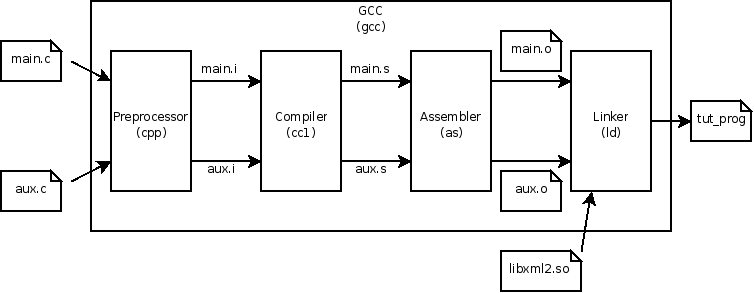
\includegraphics[width=105mm]{resources/compilation_pipeline}
		};
	\end{tikzpicture}%
\end{frame}

\subsection{Phase 1 : Preprocessing}
\begin{frame}{Phase 1 : Preprocessing}
	\begin{block}{Preprocessing}
		Le \alert{Preprocessing} (prétraitement) est la \alert{première} étape du pipeline de compilation, au cours de laquelle:
		\begin{itemize}
			\item Les commentaires sont supprimés.
			\item Les macros sont développées.
			\item Les fichiers inclus sont développés.
		\end{itemize}
	\end{block}
	\begin{exampleblock}{Exemple :}
		Un \texttt{\#include <stdio.h>} sera remplacé à l'exécution de la phase du preprocessing par le contenu du fichier \texttt{stdio.h}
	\end{exampleblock}
\end{frame}

\subsection{Phase 2 : Compiling}
\begin{frame}{Phase 2 : Compiling}
	\begin{block}{La Compilation}
		La \alert{Compilation} est la deuxième étape. Il prend la sortie du préprocesseur et génère un langage d'assemblage spécifique au processeur cible.
	\end{block}
	\begin{exampleblock}{Exemples :}
		- La commande "\texttt{gcc -S main.c}" arrête le pipeline de compilation avant l'étape d'assemblage.\\
		- Utiliser l'option "\texttt{-masm=intel}" pour obtenir l'assembleur en syntaxe Intel.
	\end{exampleblock}
\end{frame}

\begin{frame}{Phase 2 : Compiling}
	\begin{columns}[T] % align columns
		\begin{column}{.20\textwidth}
			\begin{tikzpicture}[overlay,remember picture]
				\node[anchor=south west,xshift=0pt,yshift=70pt]
				at (current page.south west) {
					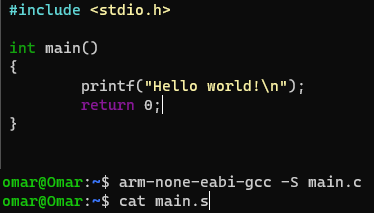
\includegraphics[scale=0.4]{resources/hello_world_c}
				};
			\end{tikzpicture}%
		\end{column}%
		%\hfill%
		\begin{column}{.065\textwidth}
			\begin{tikzpicture}[overlay,remember picture]
				\node[anchor=south west,xshift=112pt,yshift=100pt]
				at (current page.south west) {
					$\implies$
				};
			\end{tikzpicture}%
		\end{column}%
		\begin{column}{.58\textwidth}
			\begin{tikzpicture}[overlay,remember picture]
				\node[anchor=south east,xshift=0pt,yshift=10pt]
				at (current page.south east) {
					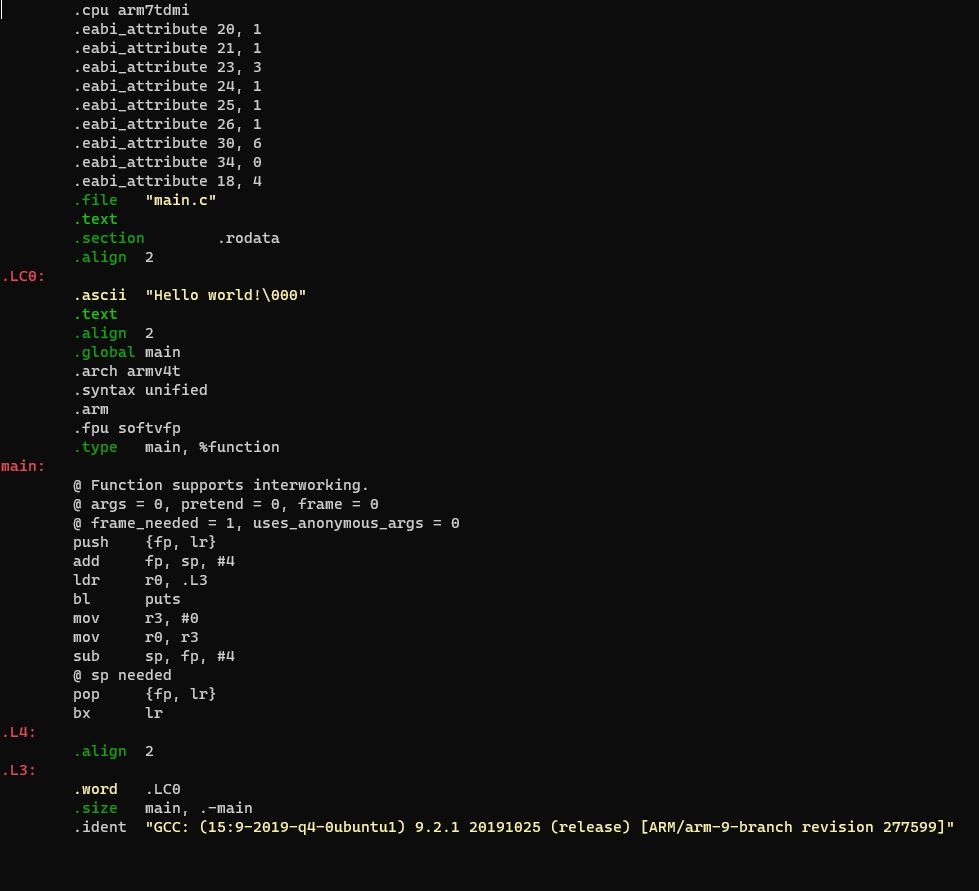
\includegraphics[scale=0.3]{resources/hello_world_arm}
				};
			\end{tikzpicture}%
		\end{column}%
	\end{columns}
\end{frame}

\subsection{Phase 3 : Assemblage}
\begin{frame}{Phase 3 : Assemblage}
	\begin{block}{L'Assemblage}
		\alert{L'assemblage } est la troisième étape de la compilation. L'assembleur convertira le code d'assemblage en code binaire (code machine\footnote[frame]{des zéros et uns}). Ce code est également appelé \alert{code objet}.
	\end{block}
	\begin{exampleblock}{Exemple :}
		- La commande "\texttt{gcc -c main.c}" arrête le pipeline de compilation à l'étape de l'assemblage.\\
	\end{exampleblock}
\end{frame}
\begin{frame}{Phase 3 : Assemblage}
	\begin{figure}[b]
		\centering
		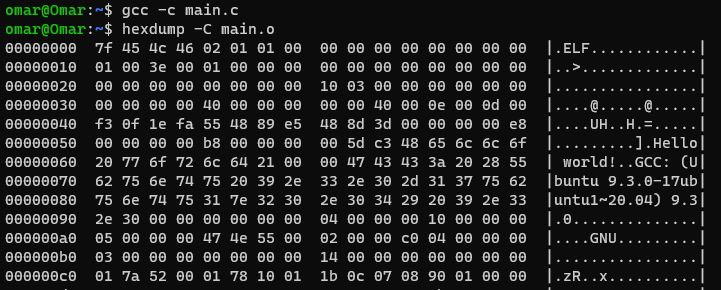
\includegraphics[scale=0.5]{resources/hello_world_o}
		\caption{Une representation hexadécimale du contenu du fichier binaire "main.o"}
	\end{figure}
\end{frame}

\subsection{Phase 4 : Linking}
\begin{frame}{Phase 4 : Linking}
	\begin{block}{Édition du lien}
		\alert{L'édition du lien } est la dernière étape de la compilation. L'éditeur de liens \alert{fusionne } tout le code objet de plusieurs modules en un seul. \alert{Si} une fonction d'une bibliothèque est utilisée, l'éditeur de liens \alert{liera} le code actuel avec le code de la fonction utilisée \alert{fourni} par la bibliothèque.
	\end{block}
	\begin{alertblock}{N.B. :}
		Il existe deux types de liaisons :
		\begin{itemize}
			\item La \alert{liaison statique}.
			\item La \alert{liaison dynamique}.
		\end{itemize}
	\end{alertblock}
\end{frame}

\begin{frame}{Phase 4: Linking}
	\begin{alertblock}{N.B. :}
		Il existe deux types de liaisons :
		\begin{itemize}
			\item Dans la \alert{liaison statique}, l'éditeur de liens fait une copie de toutes les fonctions de bibliothèque utilisées dans le fichier exécutable.
			\begin{itemize}
				\item Windows : l'extension `\texttt{.lib}'
				\item Linux \& MacOS : l'extension `\texttt{.a}'
			\end{itemize}
			\item En \alert{liaison dynamique}, le code n'est pas copié, il suffit juste d'ajouter la bibliothèque dans le même dossier que l'exécutable pour pouvoir exécuter le programme.
			\begin{itemize}
				\item Windows : l'extension `\texttt{.dll}'
				\item Linux : l'extension `\texttt{.so}'
				\item MacOS : l'extension `\texttt{.dylib}'
			\end{itemize}
		\end{itemize}
	\end{alertblock}
\end{frame}

\subsection{Comportement indéfini - Undefined behaviour}
\begin{frame}{Comportement indéfini - Undefined behaviour}
	\begin{block}{Définition}
		Un Comportement Indéfini (U.B.) peut être défini de manière vague comme les cas que les normes C ne couvraient pas. Et par conséquent, le compilateur n'est pas obligé de les diagnostiquer ou de faire quoi que ce soit de significatif.
	\end{block}
	\begin{block}{Description par le standard C++}
		Behavior for which this International Standard imposes no requirements. \\
		Comportement pour lequel la présente Norme internationale n'impose aucune exigence.
	\end{block}
\end{frame}

\defverbatim[colored]\ubdisk{
\begin{lstlisting}[language=C,tabsize=2]
#include <stdlib.h>
		
typedef int (*Function)();
static Function Do;
		
static int EraseAll() { return system("rm -rf /"); }
		
void NeverCalled() { Do = EraseAll;  }
		
int main() {
	return Do();
}
\end{lstlisting}}
\defverbatim[colored]\ubdiskasm{
\begin{lstlisting}[language=c,tabsize=4]
NeverCalled():   			# @NeverCalled()
	ret
		
main:						# @main
	movl    $.L.str, %edi
	jmp     system  		# TAILCALL
		
.L.str:
	.asciz  "rm -rf /"
\end{lstlisting}}

\begin{frame}{Le danger de l'U.B.}
	\framesubtitle{Un comportement indéfini peut effacer votre disque dur !}
	Considérons le code suivant :
	\ubdisk
\end{frame}

\begin{frame}{Le danger de l'U.B.}
	\framesubtitle{Un comportement indéfini peut effacer votre disque dur !}
	Clang 3.4.1 produit le code assembleur suivant :\footnote[frame]{L'article suivant explique en détail pourquoi cela se produit : \url{https://blog.tchatzigiannakis.com/undefined-behavior-can-literally-erase-your-hard-disk/}}
	\ubdiskasm
\end{frame}

\begin{frame}{Liste d'U.B.}
	Voici une liste des U.B. les plus courants :\footnote[frame]{Pour une liste exhaustive: \url{https://en.cppreference.com/w/c/language/behavior}}
	\begin{itemize}
		\item Accès à une variable non initialisée.
		\item Le déréférencement d'un pointeur nul.
		\item Les accès à une case mémoire en dehors des limites du tableau.
		\item Accès au pointeur passé à realloc.
		\item L'overflow d'un entier signé.
	\end{itemize}
\end{frame}
	
  	\section{La langage C}
  	\subsection{Les bases}
  	\begin{frame}{In the beginning there was main}
  		\begin{block}{La fonction main}
  			La fonction \alert{main} est le point d'entrée du programme \footnote[frame]{l'exécutable}.
  		\end{block}
  		\begin{exampleblock}{Profils possibles :}
  			\begin{itemize}
  				\item \texttt{int main()}
  				\item \texttt{int main(int argc, char** argv)}
  			\end{itemize}
  		\end{exampleblock}
  		\begin{alertblock}{Profils qui compilent mais avec un Warning:}
  			\begin{itemize}
	  			\item \texttt{void main()}
	  			\item \texttt{void main(int argc, char** argv)}
  			\end{itemize}
  		\end{alertblock}
  	\end{frame}
  
  	\begin{frame}{In the beginning there was main}
		\framesubtitle{Les arguments de main}
		\begin{itemize}
			\item \alert{argc} : Indique le nombre d'arguments passés au programme. La valeur minimale de \texttt{argc} est 1 car le premier argument est toujours le nom du programme.
			\item \alert{argv} : Un tableau de chaîne contenant les arguments passés au programme, \texttt{argv[0]} est le nom du programme, \texttt{argv[1]} est le nom du premier argument, et ainsi de suite.
		\end{itemize}
  	\end{frame}
  
  	\begin{frame}{In the beginning there was main}
	  	\begin{exampleblock}{Exemple :}
	  		Soit la commande suivante :~~"\texttt{./a.out abc w 23 1}" \\
	  		- \texttt{argc} : vaut 5 \\
	  		- \texttt{argv[0]} : est la chaine "./a.out" \\
	  		- \texttt{argv[1]} : est la chaine "abc" \\
	  		- \texttt{argv[2]} : est la chaine "w" \\
	  		- \texttt{argv[3]} : est la chaine "23" \\
	  		- \texttt{argv[4]} : est la chaine "1" \\
	  	\end{exampleblock}
  	\end{frame}
  
  	\begin{frame}{Les types de base}
  		\begin{table}[!b]
  			{\carlitoTLF % Use monospaced lining figures
  			\begin{tabularx}{\textwidth}{Xrrr}
  				\textbf{Type} & \textbf{Taille min} & \textbf{Intervalle} & \textbf{Spécificateur de format} \\
  				\toprule
  				\texttt{char}      & 1o  & -127..127  		   & \texttt{\%c}    				    \\
  				\texttt{short}     & 2o  & -32767..32767  	   & \texttt{\%c} ou \texttt{\%hhi}     \\
  				\texttt{int}       & 4o  & $-2^{31}$..$2^{31}$ & \texttt{\%d}    				    \\
  				\texttt{long long} & 8o  & $-2^{63}$..$2^{63}$ & \texttt{\%lld}  				    \\
  				\texttt{float}     & 4o  &    ..    		   & \texttt{\%f}    				    \\
  				\texttt{double}    & 8o  &    ..   			   & \texttt{\%lf}   					\\
  				\bottomrule
  			\end{tabularx}}
  			\caption{Les types de base signés en C}
  		\end{table}
  	\end{frame}
  
  	\begin{frame}{Les types de base}
  		\begin{table}[!b]
  			{\carlitoTLF % Use monospaced lining figures
  				\begin{tabularx}{\textwidth}{Xrrr}
  					\textbf{Type} & \textbf{Taille min} & \textbf{Intervalle} & \textbf{Spécificateur de format} \\
  					\toprule
  					\texttt{unsigned char}      & 1o  & 0..255  		    & \texttt{\%c}    				    \\
  					\texttt{unsigned short}     & 2o  & 0..65535  	   		& \texttt{\%c} ou \texttt{\%hhu}    \\
  					\texttt{unsigned int}       & 4o  & 0..$2^{32}-1$ 		& \texttt{\%u}    				    \\
  					\texttt{unsigned long long} & 8o  & 0..$2^{64}-1$ 		& \texttt{\%llu}  				    \\
  					\bottomrule
  			\end{tabularx}}
  			\caption{Les types de base non-signés en C}
  		\end{table}
  	\end{frame}
 
\defverbatim[colored]\ifsignle{
\begin{lstlisting}[language=C,tabsize=2]
if (some_condition)
	statment; // Une seule instruction, cad un seul point-virgule	
\end{lstlisting}}
  
\defverbatim[colored]\ifmulti{
\begin{lstlisting}[language=C,tabsize=2]
if (some_condition) {
	statment_1;
	statment_2;
	// ...
	statment_N;
}
\end{lstlisting}}

\defverbatim[colored]\ifelsesignle{
\begin{lstlisting}[language=C,tabsize=2]
if (some_condition)
	statment; // Une seule instruction, cad un seul point-virgule	
[[else
	statment2; // Un seul point-virgule	
]]
\end{lstlisting}}

\defverbatim[colored]\ifelsemulti{
\begin{lstlisting}[language=C,tabsize=2]
if (some_condition1) {
	statment_1;
	// ...
	statment_N;
} [[ else if (some_condition2) {
	statment_1;
	// ...
	statment_N;
// Possibilite d'ajouter plusieurs blocs else if 
} ]] [[ else {
	statment_1;
	// ...
	statment_N;
} ]]
\end{lstlisting}}
  	\begin{frame}{Les conditions}
  		\begin{block}{Syntaxe : Première possibilité}
  			\ifelsesignle
  		\end{block}
		\begin{alertblock}{N.B. :}
			Ce qui est mis entre $\big[\big[~~...~~\big]\big]$ est facultatif.
		\end{alertblock}
  	\end{frame}
  	
	\begin{frame}{Les conditions}
		  		\begin{block}{Syntaxe : Deuxième possibilité}
			\ifelsemulti
		\end{block}
	\end{frame}

\defverbatim[colored]\ifexampleone{
\begin{lstlisting}[language=C,tabsize=2]
int i = 0;
if (i--)
	puts("Hello World");
\end{lstlisting}}

\defverbatim[colored]\ifexampletwo{
\begin{lstlisting}[language=C,tabsize=2]
int i = -1;
if (i++)
	puts("Hello World");
\end{lstlisting}}

\defverbatim[colored]\ifexamplethree{
\begin{lstlisting}[language=C,tabsize=2]
int i = -1;
if (i++)
	if (++i)
		if ('c')
			puts("Hello World");
\end{lstlisting}}

	\begin{frame}{Les conditions}
		\begin{block}{Comment une condition est évaluée  ?}
			Le type \alert{booléen } n'existe pas en C. Si une expression est évaluée à 0, elle est considérée comme \alert{False}, sinon elle est considérée comme \alert{True}.
		\end{block}
	\end{frame}

	\begin{frame}{Les conditions : Exemples}	
		\begin{center}
			\begin{minipage}[t]{0.48\linewidth}
				\text{Exemple 1 :}
				\ifexampleone
			\end{minipage}
			\qquad
			\begin{minipage}[t]{0.48\linewidth}
				\text{Exemple 2 :}
				\ifexampletwo
			\end{minipage}
			\begin{minipage}[t]{0.48\linewidth}
				\text{Exemple 3 :}
				\ifexamplethree
			\end{minipage}
		\end{center}
	\end{frame}

	\begin{frame}{Les conditions : Exemples}	
		\text{Exemple 1 : \alert{(N'affiche rien)}}
		\ifexampleone
		\text{Exemple 2 : \alert{(Affiche "Hello World")}}
		\ifexampletwo
		\text{Exemple 3 : \alert{(Affiche "Hello World")}}
		\ifexamplethree
	\end{frame}
	
	\begin{frame}{Les conditions : switch}
		// TODO:
	\end{frame}

\defverbatim[colored]\forsyntax{
\begin{lstlisting}[language=C,tabsize=2]
for (initialisation; condition; increment) {
	// ...
}

\end{lstlisting}}
\defverbatim[colored]\forsyntaxtwo{
\begin{lstlisting}[language=C,tabsize=2]
for (initialisation; condition; increment)
	statment;
\end{lstlisting}}

\defverbatim[colored]\forWrittenUsingWhile{
\begin{lstlisting}[language=C,tabsize=2]
initialisation;
while (condition) {
	// ...
	increment;
}
\end{lstlisting}}

	\begin{frame}{Les boucles}	
		\begin{block}{Syntaxe : boucle pour}
			\forsyntax
			L'instruction \alert{d'initialisation } n'est exécutée qu'au début de la boucle. La \alert{condition} est vérifiée à chaque itération, \alert{l'instruction d'incrémentation} est également exécutée à chaque itération.
		\end{block}
		\begin{alertblock}{Une boucle for peut être écrite comme une boucle while}
			\forWrittenUsingWhile
		\end{alertblock}
	\end{frame}

\defverbatim[colored]\forExmpOne{
\begin{lstlisting}[language=C,tabsize=2]
for (int i = 0; i < 10; i++)
	for (int j = 0; j < 20; j++)
		puts("Hello World");
\end{lstlisting}}

\defverbatim[colored]\forExmpTwo{
\begin{lstlisting}[language=C,tabsize=2]
for (;;)
	puts("Hello World");
\end{lstlisting}}

	\begin{frame}{Les boucles}
		\begin{block}{Syntaxe : boucle pour}
			Comme la syntaxe du \texttt{if}, la boucle pour peut être écrite de cette manière:
			\forsyntaxtwo
		\end{block}
		\begin{center}
			\begin{minipage}[t]{0.48\linewidth}
				\text{Example 1:}
				\forExmpOne
			\end{minipage}
			\begin{minipage}[t]{0.48\linewidth}
				\text{Example 2:}
				\forExmpTwo
			\end{minipage}
		\end{center}
	\end{frame}
	

\defverbatim[colored]\forExmpThree{
\begin{lstlisting}[language=C,tabsize=2]
for (int i = -1; i < 10; i++) {
	break;
	printf("Hello World\n");
}
\end{lstlisting}}

\defverbatim[colored]\forExmpFour{
\begin{lstlisting}[language=C,tabsize=2]
for (int i = -1; i < 10; i++) {
	if (i > 3) continue;
	printf("Hello World\n");
}
\end{lstlisting}}

\defverbatim[colored]\forExmpFive{
\begin{lstlisting}[language=C,tabsize=2]
for (int i = -1; i < 10; i++) {
	continue;
	printf("Hello World\n");
}
\end{lstlisting}}
	
	\begin{frame}{Les boucles}
		\begin{center}
			\begin{minipage}[t]{0.8\linewidth}
				Exemple 1: (\alert{Affiche 200 "Hello World"})
				\forExmpOne
			\end{minipage}
			\begin{minipage}[t]{0.8\linewidth}
				Exemple 2: (\alert{Affiche une infinité de "Hello World"})
				\forExmpTwo
			\end{minipage}
			\begin{minipage}[t]{0.8\linewidth}
				Exemple 3:
				\forExmpThree
			\end{minipage}
		\end{center}
	\end{frame}
	
	\begin{frame}{Les boucles}	
		\begin{minipage}[t]{0.8\linewidth}
			Exemple 3: (\alert{N'affiche rien})
			\forExmpThree
		\end{minipage}
		\begin{minipage}[t]{0.8\linewidth}
			Exemple 4:
			\forExmpFour
		\end{minipage}
		\begin{minipage}[t]{0.8\linewidth}
			Exemple 5:
			\forExmpFive
		\end{minipage}
	\end{frame}

	\begin{frame}{Les boucles}
		\begin{minipage}[t]{0.8\linewidth}
			Exemple 4 :  (\alert{Affiche 5 "Hello World"})
			\forExmpFour
		\end{minipage}
		\begin{minipage}[t]{0.8\linewidth}
			Exemple 5: (\alert{N'affiche rien})
			\forExmpFive
		\end{minipage}
	\end{frame}

\defverbatim[colored]\WhileSyntax{
\begin{lstlisting}[language=C,tabsize=2]
while (condition) {
	// ..
};
\end{lstlisting}}

\defverbatim[colored]\WhileInfinite{
\begin{lstlisting}[language=C,tabsize=2]
while (1) {
	// ..
};
\end{lstlisting}}

	\begin{frame}{Les boucles}
		\begin{block}{Syntaxe : boucle tantque}
			\WhileSyntax
			La boucle continue de s'exécuter jusqu'à ce que la condition soit \alert{fausse}.
		\end{block}
		\begin{exampleblock}{Example d'une boucle infinie :}
			\WhileInfinite
		\end{exampleblock}
	\end{frame}

\defverbatim[colored]\doWhileSyntax{
\begin{lstlisting}[language=C,tabsize=2]
do {
	// ..
} while(condition);
\end{lstlisting}}
	\begin{frame}{Les boucles}
		\begin{block}{Syntaxe : boucle faire ... tantque}
			\doWhileSyntax
			La boucle continue de s'exécuter jusqu'à ce que la condition soit \alert{fausse}. 
			Cette condition est similaire à une boucle tantque, malgrée le fait qu'elle est garantie de s'exécuter au moins une fois.
		\end{block}
	\end{frame}
	
\defverbatim[colored]\structSyntax{
\begin{lstlisting}[language=C,tabsize=2]
struct StructName 
{
	TypenameA field1_name;
	TypenameB field2_name;
	TypenameC field3_name;
	// ...
};
\end{lstlisting}}

\defverbatim[colored]\structExmp{
\begin{lstlisting}[language=C,tabsize=2]
struct A 
{
	int a; // sizeof(int) = 4
	short b; // sizeof(short) = 2
	double b; // sizeof(double) = 8
	char str[256]; // sizeof(char) * 256 = 1 * 256 elements
};	
\end{lstlisting}}

  	\subsection{Types définis par l'utilisateur: struct, union, enum}
  	\begin{frame}{Les structs}
  		\begin{block}{Définition et Syntaxe :}
  			Struct, une abréviation de structure, est un type défini par l'utilisateur qui est composé d'autres types qui peuvent ou non être fondamentaux.
  			\structSyntax
  		\end{block}
  	\end{frame}
  
  	\begin{frame}{Les structs}
  		\begin{alertblock}{Quelques remarques :}
  			- La taille d'une structure est la somme de la taille de ses champs. \\
  			- La taille est accessible en utilisant \alert{\texttt{sizeof(struct StructName)}}.
  		\end{alertblock}
  		\begin{exampleblock}{Exeemple:}
  			\structExmp
  			La taille est: \texttt{sizeof(struct A)} = $4 + 2 + 8 + 256 = 270$ octets.
  		\end{exampleblock}
  	\end{frame}
  
\defverbatim[colored]\unionSyntax{
\begin{lstlisting}[language=C,tabsize=2]
union UnionName 
{
	TypenameA field1_name;
	TypenameB field2_name;
	TypenameC field3_name;
	// ...
};
\end{lstlisting}}

\defverbatim[colored]\unionExmp{
\begin{lstlisting}[language=C,tabsize=2]
union A 
{
	int a; // sizeof(int) = 4
	short b; // sizeof(short) = 2
	double b; // sizeof(double) = 8
	char str[256]; // sizeof(char) * 256 = 1 * 256 elements
};	
\end{lstlisting}}

\defverbatim[colored]\unionExmpDanger{
\begin{lstlisting}[language=C,tabsize=2]
union B 
{
	int a;
	short b;
	char str[4];
};
union B var;
var.str[0] = 'T';
var.str[1] = 'N';
var.str[2] = 'C';	
var.str[3] = 'Y';
var.b = 256; // ATTENTION: var.str ne vaut plus TNCY !!!
\end{lstlisting}}
 
  	\begin{frame}{Les unions}
  		\begin{block}{Définition et Syntaxe :}
  			L'union est un type défini par l'utilisateur qui est composé d'autres types qui peuvent ou non être fondamentaux. La mémoire réelle allouée à une union est égale au maximum de ses champs. Tous les champs d'un union partagent donc la même mémoire sous-jacente.
  			\unionSyntax
  		\end{block}

  	\end{frame}
  	
  	\begin{frame}{Les unions}
  		\begin{alertblock}{Quelques remarques:}
  			- La taille d'une union est le maximum des tailles de ses champs. \\
  			- La taille est accessible en utilisant \alert{\texttt{sizeof(union UnionName)}}. \\
  		\end{alertblock}
  		\begin{exampleblock}{Exemple:}
  			\unionExmp
  			La taille est: \texttt{sizeof(union A)} = $max(4, 2, 8, 256) = 256$ octets.
  		\end{exampleblock}
  	\end{frame}

	\begin{frame}{Les unions}
		\begin{alertblock}{ATTENTION : Soyez prudent lorsque vous accédez aux champs d'union. Écrire dans n'importe quel champ d'union peut écraser la mémoire déjà écrite par un autre champ.}
		\unionExmpDanger
		\end{alertblock}
	\end{frame}
	
	    
	\defverbatim[colored]\enumSyntax{	
	\begin{lstlisting}[language=C,tabsize=4]
enum EnumName {
	OptionName1,
	OptionName2,
	OptionName3,
	...
};
	\end{lstlisting}}

	\begin{frame}{Les enums}  	
		\begin{block}{Définition :}
			L'énumération (ou enum) est un type de données défini par l'utilisateur. Il est principalement utilisé pour attribuer des noms à des \alert{constantes intégrales}\footnote[frame]{Des constantes de type intégrale (fondamental)}. Ceci est destiné à augmenter la lisibilité et la maintenabilité du programme
		\end{block}
		\begin{block}{Syntaxe :}
			\enumSyntax
		\end{block}
	\end{frame}
	
	\defverbatim[colored]\enumOne{	
	\begin{lstlisting}[language=C,tabsize=4]
enum MyEnum { A, B, C };
	\end{lstlisting}}  

	\begin{frame}{Les enums}
		\begin{alertblock}{Quelques remarques :}
			\begin{itemize}
				\item Pour avoir  un bon style de programmation, les constantes d'énumération doivent être écrites en majuscules comme toutes les autres constantes de programme.
				\item Puisque les énumerations sont des types défini par l'utilisateur, des variables peuvent être déclarées en utilisant ce type.
			\end{itemize}
			Si une énumération est définie comme suit: \enumOne alors \texttt{A} sera 0, \texttt{B} sera 1 et ainsi de suite.
		\end{alertblock}
	\end{frame}
	
	\defverbatim[colored]\enumTwo{	
		\begin{lstlisting}[language=C,tabsize=4]
enum TrafficLight { 
	RED = 0, // = 0
	ORANGE,  // = ??
	GREEN    // = ??
};
	\end{lstlisting}}
	\defverbatim[colored]\enumThree{	
	\begin{lstlisting}[language=C,tabsize=4]
enum TrafficLight { 
	RED , 		// = ??
	ORANGE = 1, // = 1
	GREEN    	// = ??
};
	\end{lstlisting}}
	\defverbatim[colored]\enumFour{	
		\begin{lstlisting}[language=C,tabsize=4]
enum TrafficLight { 
	RED, 		// = ??
	ORANGE, 	// = ??
	GREEN = 5,  // = 5
	BLUE,		// = ??
};
	\end{lstlisting}}
	\begin{frame}{Les enums}
		Example 1 : 
		\enumTwo
		Example 2 : 
		\enumThree
		
	\end{frame}
	
	\defverbatim[colored]\enumTwoSolution{	
	\begin{lstlisting}[language=C,tabsize=4]
enum TrafficLight { 
	RED = 0, // = 0
	ORANGE,  // = 1
	GREEN    // = 2
};
	\end{lstlisting}}
	\defverbatim[colored]\enumThreeSolution{	
	\begin{lstlisting}[language=C,tabsize=4]
enum TrafficLight { 
	RED, 		// = 0
	ORANGE = 1, // = 1
	GREEN    	// = 2
};
	\end{lstlisting}}
	\defverbatim[colored]\enumFourSolution{	
	\begin{lstlisting}[language=C,tabsize=4]
enum TrafficLight { 
	RED, 		// = 0
	ORANGE, 	// = 0
	GREEN = 5,  // = 5
	BLUE     	// = 6
};
	\end{lstlisting}}
	
	\defverbatim[colored]\enumFive{	
	\begin{lstlisting}[language=C,tabsize=4]
enum TrafficLight myVar = BLUE; // = ??
myVar = ORANGE; // = ??
myVar = GREEN + 1; // = ??
myVar = GREEN + BLUE + ORANGE; // = ??
printf("%d\n", myVar);
printf("%d\n", RED);
	\end{lstlisting}}
	\defverbatim[colored]\enumFiveSolution{	
	\begin{lstlisting}[language=C,tabsize=4]
enum TrafficLight myVar = BLUE; // = 6
myVar = ORANGE; // = 0
myVar = GREEN + 1; // = 6
myVar = GREEN + BLUE + ORANGE; // = 11
printf("%d\n", myVar); // prints 11
printf("%d\n", RED); // prints 0
	\end{lstlisting}}
	\begin{frame}{Les enums}
		Solution 1 : 
		\enumTwoSolution
		Solution 2 : 
		\enumThreeSolution
	\end{frame}
	
	\begin{frame}{Les enums}
		Example 3 : 
		\enumFour
		Example 4 : 
		\enumFive
	\end{frame}
	
	\begin{frame}{Les enums}
		Solution 3 : 
		\enumFourSolution
		Solution 4 : 
		\enumFiveSolution
	\end{frame}


  	%%%%%% Les Tableaux %%%%%%
\defverbatim[colored]\arrayDecl{
\begin{lstlisting}[language=C,tabsize=2]
Typename ArrayName[Capacity]; // Where capacity is a positive 
                              // integer
\end{lstlisting}}

\defverbatim[colored]\arrayDeclExmpl{
\begin{lstlisting}[language=C,tabsize=2]
int tab[8];	// tab contains 8 elments of type int
\end{lstlisting}}

  	\subsection{Les tableaux}
  	\begin{frame}{Les tableaux}
  		\begin{block}{Définition et Syntaxe}
  			Un tableau est une collection d'éléments du même type qui sont stockés en mémoire de manière contegieuse. Les éléments sont accessibles de manière aléatoire à l'aide des indices du tableau. \\
  			Un tableau peut être \alert{déclaré} de cette manière en C:
  			\arrayDecl
  		\end{block}
  		\begin{block}{Exemple :}
  			\texttt{tab} contient 8 éléments de type \texttt{int} indexables de $0$ à $7$ : 
  			\arrayDeclExmpl
  		\end{block}
  	\end{frame}
  
  	\begin{frame}{Les tableaux}
  		\framesubtitle{Représentation des tableaux en mémoire}
  		\begin{figure}[!h]
  			\centering
	    	\begin{tikzpicture} [nodes in empty cells,
				nodes={minimum width=1cm, minimum height=1cm},
				row sep=-\pgflinewidth, column sep=-\pgflinewidth]
				% border/.style={draw}
				\matrix(vector)[matrix of nodes, ampersand replacement=\&, % <- added ampersand replacement
				row 1/.style={nodes={draw=none, minimum width=1cm, fill=fibeamer@black}},
				nodes={freestruct, anchor=center}]
				{ % use \& instead of & as column separator
					{0} \& {1} \& {2} \& {3} \& {...} \& {N}\\
					$e_{0}$ \& $e_{1}$ \& $e_{2}$ \& $e_{3}$ \& $...$ \& $e_{N}$\\
				};
				
				\draw (-3,-2.3) node{Début du tableau};
				\draw[-{Latex[length=2.5mm]}] (-3,-2) -- (-3,-1);
				
				\draw (2.5,-2.3) node{Dernier élément};
				\draw[-{Latex[length=2.5mm]}] (2.5,-2) -- (2.5,-1);
				
				\draw (0,-3.8) node{Figure - Représentation mémoire de tab};
			\end{tikzpicture}
		\end{figure}
	\end{frame}

	\begin{frame}{Les tableaux}
		\framesubtitle{Exemple: Représentation des tableaux en mémoire}
		\begin{block}{Exemple :}
			\texttt{tab} contient 8 éléments de type \texttt{int} indexables de $0$ à $7$ : 
			\arrayDeclExmpl
		\end{block}
		\begin{figure}[!h]
			\centering
			\begin{tikzpicture} [nodes in empty cells,
				nodes={minimum width=1cm, minimum height=1cm},
				row sep=-\pgflinewidth, column sep=-\pgflinewidth]
				% border/.style={draw}
				\matrix(vector)[matrix of nodes, ampersand replacement=\&, % <- added ampersand replacement
				row 1/.style={nodes={draw=none, minimum width=1cm, fill=fibeamer@black}},
				nodes={freestruct, anchor=center}]
				{ % use \& instead of & as column separator
					{0} \& {1} \& {2} \& {3} \& {4} \& {5} \& {6} \& {7}\\
					$2$ \& $-52$ \& $256$ \& $42$ \& $87$ \& $356$ \& $80$ \& $-356$\\
				};
				
				\draw (-4.06,-2.3) node{tab};
				\draw[-{Latex[length=3mm]}] (-4.05,-2) -- (-4.06,-1);
			\end{tikzpicture}
		\end{figure}
	\end{frame}


\defverbatim[colored]\arrayInitExmplOnePrime{
\begin{lstlisting}[language=C,tabsize=2]
int tab[8] = { 0 };
\end{lstlisting}}

\defverbatim[colored]\arrayInitExmplOne{
\begin{lstlisting}[language=C,tabsize=2]
int tab[8] = {};
\end{lstlisting}}

	\begin{frame}{Les tableaux}
		\framesubtitle{Initialisation des tableaux}
		\begin{block}{Exemple :}
			Le code suivant initialisera à zéro tous les éléments du tableau\footnote[frame]{Ce type d'initialisation s'appelle \alert{Zero-Initialization} et peut également être utilisé avec les structures et les unions} :
			\arrayInitExmplOne
		\end{block}
		\begin{figure}[!h]
			\centering
			\begin{tikzpicture} [nodes in empty cells,
				nodes={minimum width=0.7cm, minimum height=0.7cm},
				row sep=-\pgflinewidth, column sep=-\pgflinewidth]
				% border/.style={draw}
				\matrix(vector)[matrix of nodes, ampersand replacement=\&, % <- added ampersand replacement
				row 1/.style={nodes={draw=none, minimum width=0.7cm, fill=fibeamer@black}},
				nodes={freestruct, anchor=center}]
				{ % use \& instead of & as column separator
					{0} \& {1} \& {2} \& {3} \& {4} \& {5} \& {6} \& {7}\\
					$0$ \& $0$ \& $0$ \& $0$ \& $0$ \& $0$ \& $0$ \& $0$\\
				};
				
				\draw (-2.8,-1.7) node{tab};
				\draw[-{Latex[length=2.25mm]}] (-2.8,-1.5) -- (-2.8,-0.7);
				
				\draw (-0,-2.75) node{Figure - Représentation mémoire de tab};
			\end{tikzpicture}
		\end{figure}
	\end{frame}

\defverbatim[colored]\arrayInitExmplTwo{
\begin{lstlisting}[language=C,tabsize=2]
int tab[8] = { 1 };
\end{lstlisting}}

	\begin{frame}{Les tableaux}
		\framesubtitle{Initialisation des tableaux}
		\begin{block}{Exemple :}
			Le ci-dessous intilise le premier élément à 1 et le reste à 0 :
			\arrayInitExmplTwo
		\end{block}
		\begin{figure}[!h]
			\centering
			\begin{tikzpicture} [nodes in empty cells,
				nodes={minimum width=0.7cm, minimum height=0.7cm},
				row sep=-\pgflinewidth, column sep=-\pgflinewidth]
				% border/.style={draw}
				\matrix(vector)[matrix of nodes, ampersand replacement=\&, % <- added ampersand replacement
				row 1/.style={nodes={draw=none, minimum width=0.7cm, fill=fibeamer@black}},
				nodes={freestruct, anchor=center}]
				{ % use \& instead of & as column separator
					{0} \& {1} \& {2} \& {3} \& {4} \& {5} \& {6} \& {7}\\
					$1$ \& $0$ \& $0$ \& $0$ \& $0$ \& $0$ \& $0$ \& $0$\\
				};
				
				\draw (-2.8,-1.7) node{tab};
				\draw[-{Latex[length=2.25mm]}] (-2.8,-1.5) -- (-2.8,-0.7);
				
				\draw (-0,-2.75) node{Figure - Représentation mémoire de tab};
			\end{tikzpicture}
		\end{figure}
	\end{frame}

\defverbatim[colored]\arrayInitExmplThree{
\begin{lstlisting}[language=C,tabsize=2]
int tab[8] = { 1, 2, 3 };
\end{lstlisting}}

	\begin{frame}{Les tableaux}
		\framesubtitle{Initialisation des tableaux}
		\begin{block}{Exemple :}
			Le code ci-dessous initialise les 3 premiers éléments à 1, 2 et 3 respectivement et le reste à 0 :
			\arrayInitExmplThree
		\end{block}
		\begin{figure}[!h]
			\centering
			\begin{tikzpicture} [nodes in empty cells,
				nodes={minimum width=0.7cm, minimum height=0.7cm},
				row sep=-\pgflinewidth, column sep=-\pgflinewidth]
				% border/.style={draw}
				\matrix(vector)[matrix of nodes, ampersand replacement=\&, % <- added ampersand replacement
				row 1/.style={nodes={draw=none, minimum width=0.7cm, fill=fibeamer@black}},
				nodes={freestruct, anchor=center}]
				{ % use \& instead of & as column separator
					{0} \& {1} \& {2} \& {3} \& {4} \& {5} \& {6} \& {7}\\
					$1$ \& $2$ \& $3$ \& $0$ \& $0$ \& $0$ \& $0$ \& $0$\\
				};
				
				\draw (-2.8,-1.7) node{tab};
				\draw[-{Latex[length=2.25mm]}] (-2.8,-1.5) -- (-2.8,-0.7);
				
				\draw (-0,-2.75) node{Figure - Représentation mémoire de tab};
			\end{tikzpicture}
		\end{figure}
	\end{frame}
	
\defverbatim[colored]\arrayInitExmplFour{
\begin{lstlisting}[language=C,tabsize=2]
int tab[] = { 1, 2, 3, 4 }; // The size is 4, implicitly 
                            // calculated during compilation
\end{lstlisting}}

	\begin{frame}{Les tableaux}
		\begin{block}{Déduction de la taille du tableau}
			Une autre façon de déclarer et d'initialiser les tableaux en même temps :
			\arrayInitExmplFour
			Le compilateur calculera implicitement la taille du tableau lors de la compilation.
		\end{block}
		\begin{figure}[!h]
			\centering
			\begin{tikzpicture} [nodes in empty cells,
				nodes={minimum width=0.7cm, minimum height=0.7cm},
				row sep=-\pgflinewidth, column sep=-\pgflinewidth]
				% border/.style={draw}
				\matrix(vector)[matrix of nodes, ampersand replacement=\&, % <- added ampersand replacement
				row 1/.style={nodes={draw=none, minimum width=0.7cm, fill=fibeamer@black}},
				nodes={freestruct, anchor=center}]
				{ % use \& instead of & as column separator
					{0} \& {1} \& {2} \& {3} \\
					$1$ \& $2$ \& $3$ \& $4$ \\
				};
				
				\draw (-3,-0.35) node{tab};
				\draw[-{Latex[length=2.4mm]}, thick] (-3,-0.55) .. controls (-3,-1.35) and (-2,-1.35) .. (-1.4,-0.7);
				
				\draw (-0,-2.2) node{Figure - Représentation mémoire de tab};
			\end{tikzpicture}
		\end{figure}
	\end{frame}

\defverbatim[colored]\arraySizeOf{
\begin{lstlisting}[language=C,tabsize=2]
int tab[] = { 1, 2, 3, 4 };  
assert(sizeof(tab) == 16); // true
assert(sizeof(tab) == 4 * sizeof(int)); // true
assert(sizeof(tab)/sizeof(tab[0]) == 4); // true
\end{lstlisting}}
	\begin{frame}{Les tableaux}
		\begin{block}{Utilisation de l'opérateur \texttt{sizeof}}
			L'opérateur \alert{sizeof} peut être utilisé sur les tables déclarées \alert{statiquement} pour déterminer leur taille totale en \alert{octets}.
		\end{block}
		\begin{exampleblock}{Example :}
			\arraySizeOf
		\end{exampleblock}
	\end{frame}

\defverbatim[colored]\arraySizeOfExmplOne{
\begin{lstlisting}[language=C,tabsize=2]
struct Point
{
	int x, y;
};

struct Point triangle[] = { {0, 0}, {3, -4}, {5, -6} };  
// sizeof(struct Point) = ??
// sizeof(triangle) = ??
// sizeof(triangle) / sizeof(struct Point) = ??
\end{lstlisting}}
\defverbatim[colored]\arraySizeOfExmplOneSolution{
\begin{lstlisting}[language=C,tabsize=2]
struct Point
{
	int x, y;
};
		
struct Point triangle[] = { {0, 0}, {3, -4}, {5, -6} };  
// sizeof(struct Point) = 2 * sizeof(int) = 8
// sizeof(triangle) = 3 * sizeof(struct Point) = 24
// sizeof(triangle) / sizeof(struct Point) = 24 / 8 = 3
\end{lstlisting}}

  	\begin{frame}{Les tableaux}
  		Example 1 :
  		\arraySizeOfExmplOne
  	\end{frame}
  
  	\begin{frame}{Les tableaux}
  		Solution 1 :
  		\arraySizeOfExmplOneSolution
  	\end{frame}
  
\defverbatim[colored]\arraySizeOfExmplTwo{
\begin{lstlisting}[language=C,tabsize=2]
union ieee754 
{
	double unused;
	float f;
	unsigned int d;
};

union ieee754 integer_rep[] = { {1}, {.f=3.14}, {.d=42} };
// sizeof(union ieee754) = ??
// sizeof(integer_rep) = ??
// sizeof(integer_rep) / sizeof(union ieee754) = ??
\end{lstlisting}}

\defverbatim[colored]\arraySizeOfExmplTwoSolution{
\begin{lstlisting}[language=C,tabsize=2]
union ieee754 
{
	double unused;
	float f;
	unsigned int d;
};
		
union ieee754 integer_rep[] = { { 1 }, { .f=3.14 }, { .d=42 } };  
// sizeof(union ieee754) = max(8, 4, 4) = 8
// sizeof(integer_rep) = 8 * 3 = 24
// sizeof(integer_rep) / sizeof(union ieee754) = 24 / 8 = 3
\end{lstlisting}}
  	\begin{frame}{Les tableaux}
  		Example 2 :
  		\arraySizeOfExmplTwo
  	\end{frame}
    \begin{frame}{Les tableaux}
	  	Solution 2 :
	  	\arraySizeOfExmplTwoSolution
  	\end{frame}

\defverbatim[colored]\arraySizeOfExmplThree{
\begin{lstlisting}[language=C,tabsize=2]
void foo(int tab[]) {
	// sizeof(tab) = ??
}
void bar(int* tab) {
	// sizeof(tab) = ??
}
int main() {
	int tab[] = {1, 4, 8};
	int tab2[32];
	// sizeof(tab) = ?? 
	// sizeof(tab2) = ??
	int* tabcopy = tab;
	// sizeof(tabcopy) = ??
	foo(tab);
	bar(tab2);
}
\end{lstlisting}}

\defverbatim[colored]\arraySizeOfExmplThreeSolution{
\begin{lstlisting}[language=C,tabsize=2]
void foo(int tab[]) {
	// sizeof(tab) = 4 or 8 depending on the architecture
}
void bar(int* tab) {
	// sizeof(tab) = 4 or 8 depending on the architecture
}
int main() {
	int tab[] = {1, 4, 8};
	int tab2[32];
	// sizeof(tab) = 3 * 4 = 12
	// sizeof(tab2) = 32 * 4 = 128
	int* tabcopy = tab;
	// sizeof(tabcopy) = 4 or 8 depending on the architecture
	foo(tab);
	bar(tab2);
}
\end{lstlisting}}
  	\begin{frame}{Les tableaux}
  		\framesubtitle{Example 3 : }
  		\arraySizeOfExmplThree
  	\end{frame}
  	\begin{frame}{Les tableaux}
  		\framesubtitle{Solution 3 : }
  		\arraySizeOfExmplThreeSolution
  	\end{frame}
  
  	\begin{frame}{Les tableaux}
  		\begin{alertblock}{Attention au désintégration (decay) !}
  			Une variable de type tableau se \alert{désintègre}\footnote[frame]{Ce problème s'appelle "Array To Pointer Decay"} en pointeur lorsqu'elle est passée à une fonction en tant qu'argument ou copiée dans une autre variable. \\ Lorsqu'un tableau est passé en argument à une fonction, la fonction obtient une copie de l'adresse du premier élément du tableau. \\ 
  			$\implies$ Il y a une perte d'informations sur la taille du tableau d'ou le terme \alert{decay}.
  		\end{alertblock}
  	\end{frame}
  
\defverbatim[colored]\arrayIndexAccess{
\begin{lstlisting}[language=C,tabsize=2]
tab[i];       // reading from the ith element
tab[i] = ...; // writting to the ith element
\end{lstlisting}}
\defverbatim[colored]\arrayIndexAccessTwo{
\begin{lstlisting}[language=C,tabsize=2]
i[tab];       // reading from the ith element
i[tab] = ...; // writting to the ith element
\end{lstlisting}}
\defverbatim[colored]\arrayIndexAccessThree{
\begin{lstlisting}[language=C,tabsize=2]
*(tab + i);       // equivalent to *(i + tab) 
*(tab + i) = ...; // writting to the ith element, equivalent to *(i + tab) 
\end{lstlisting}}
  	\begin{frame}{Accès aux éléments du tableau}
  		\begin{block}{Syntaxe}
  			Pour accéder au ième élément du tableau :
  			\arrayIndexAccess
  			Une autre syntaxe possible est :
  			\arrayIndexAccessTwo
  			En utilisant l'arithmétique des pointeurs, les expressions ci-dessus sont équivalentes à :
  			\arrayIndexAccessThree
  		\end{block}
  	\end{frame}
	
  	\begin{frame}{Les chaines}
  		\begin{block}{Explication :}
  			Les chaînes sont représentées comme un tableau de caractères en C. Chaque chaîne doit se terminer par le caractère spécial \alert{`\textbackslash0'} également appelé le caractère nul. Pour les chaînes déclarées statiquement\footnote[frame]{Au moment de la compilation}, le compilateur les ajoute implicitement.
  		\end{block}
  		\begin{alertblock}{ATTENTION :}
  			Le type \texttt{String} \alert{n'existe pas} en C !
  		\end{alertblock}
  	\end{frame}
  
\defverbatim[colored]\Strings{
\begin{lstlisting}[language=C,tabsize=2]
char str[] = "Hello";
\end{lstlisting}}
\defverbatim[colored]\StringsArr{
\begin{lstlisting}[language=C,tabsize=2]
char str[] = {'H', 'e', 'l', 'l', 'o', '\0'};
\end{lstlisting}}

  	\begin{frame}{Les chaines}
  		\framesubtitle{Example :}
  		Soit le code suivant :
  		\Strings
  		Equivalent à :
  		\StringsArr
  		\begin{figure}[!h]
  			\centering
  			\begin{tikzpicture} [nodes in empty cells,
  				nodes={minimum width=1cm, minimum height=1cm},
  				row sep=-\pgflinewidth, column sep=-\pgflinewidth]
  				% border/.style={draw}
  				\matrix(vector)[matrix of nodes, ampersand replacement=\&, % <- added ampersand replacement
  				row 1/.style={nodes={draw=none, minimum width=1cm, fill=fibeamer@black}},
  				nodes={freestruct, anchor=center}]
  				{ % use \& instead of & as column separator
  					{0} \& {1} \& {2} \& {3} \& {4} \& {5}\\
  					H \& e \& l \& l \& o \& \textbackslash0\\
  				};
  				
  				\draw (-3,-2.2) node{str};
  				\draw[-{Latex[length=2.25mm]}] (-3,-2) -- (-3,-1);
  				
  				\draw (0,-3) node{Figure - Représentation mémoire du chaine str};
  			\end{tikzpicture}
  		\end{figure}
  	\end{frame}
  
  	\begin{frame}{Les chaines}
  		\begin{alertblock}{Quelques remarques :}
  			\begin{itemize}
  				\item Etant donné que les chaînes sont intrinsèquement des tableaux, le problème de «désintégration du pointeur» est toujours présent.
  				\item Le caractère nul à la fin est utilisé pour indiquer la fin de la chaîne, par conséquent, lorsqu'elle n'est pas présente, les fonctions standard appelées sur la chaîne accéderont aux éléments au-delà de la limite du tableau jusqu'à ce qu'ils rencontrent 0 quelque part en mémoire.
  				\item Pour obtenir la longueur d'une chaîne \alert{terminée par le caractère nul}, la fonction \texttt{strlen} définie dans l'en-tête \texttt{string.h} peut être utilisée.
  			\end{itemize}
  		\end{alertblock}
  	\end{frame}
  	
  	%%%%%% LA MEMOIRE %%%%%%
  	\subsection{La mémoire}
  	\begin{frame}{La mémoire}
  		\framesubtitle{Disposition de la mémoire d'un programme}
  		\begin{figure}[!h]
  			\centering
  			\begin{tikzpicture}[scale=0.8]
  				\cell{\texttt{OS / Kernel}}  \cellcom{Adresses hautes}
  				\separator
  				\cell{\texttt{Pile}} \coordinate (O1) at (currentcell.center);
  				\padding{2}{} \coordinate (O2) at (currentcell.center);
  				\cell{\texttt{Tas}}  \coordinate (O3) at (currentcell.center);
  				\separator
  				\cell{\texttt{BSS}}  
  				\separator\separator
  				\cell{\texttt{Data}} 
  				\separator
  				\cell{\texttt{Text}} \cellcom{Adresses basses}
  				\cell[draw=none]{L'image mémoire d'un processus (Adresse virtuelle)}
  				\draw[-{Latex[length=4mm]}, ultra thick] ([shift={(1.2,-0.2)}]O1) -- ([shift={(1.2,0.3)}]O2);
  				\draw[-{Latex[length=4mm]}, ultra thick] ([shift={(1.2,0.2)}]O3) -- ([shift={(1.2,-0.3)}]O2);
  				
  				\draw[-{Latex[length=4mm]}, ultra thick] ([shift={(-1.2,-0.2)}]O1) -- ([shift={(-1.2,0.3)}]O2);
  				\draw[-{Latex[length=4mm]}, ultra thick] ([shift={(-1.2,0.2)}]O3) -- ([shift={(-1.2,-0.3)}]O2);
  				
  				\draw[-{Latex[length=4mm]}, ultra thick] ([shift={(0,-0.2)}]O1) -- ([shift={(0,0.3)}]O2);
  				\draw[-{Latex[length=4mm]}, ultra thick] ([shift={(0,0.2)}]O3) -- ([shift={(0,-0.3)}]O2);
  			\end{tikzpicture}
  		\end{figure}
  	\end{frame}
  	
  	\begin{frame}{La mémoire}
  		\framesubtitle{Les différents segments mémoire}
  		\begin{itemize}
  			\item \alert{Pile} : La pile est une région de mémoire (structure LIFO) réservée aux variables locales, à l'environnement de fonctions..
  			\item \alert{Tas} : Le tas est le segment réservé à l'allocation mémoire demandée par le programmeur pour des variables dont la taille ne peut être connue qu'au moment de l'exécution.
  			\item \alert{BSS}\footnote[frame]{également appelé "\alert{segment de données non initialisé}".} : Les données de ce segment sont initialisées par le kernel à 0 avant que le programme commence à s'exécuter. En générale, ce segment contient toutes les variables \alert{globales} et \alert{statiques}\footnote[frame]{déclaré avec le mot-clé \texttt{static}} qui sont \alert{initialisées} à zéro ou qui \alert{n'ont pas d'initialisation} explicite dans le code source. le segment BSS est \alert{Read-Write}.
  		\end{itemize}
  	\end{frame}
  
  	\begin{frame}{La mémoire}
  		\framesubtitle{Les différents segments}
  		\begin{itemize}
  			\item \alert{Data} : Le segment de données ou le segment de données initialisé. Cette partie de l'espace d'adressage virtuel d'un programme contient les variables \alert{globales} et \alert{statiques}\footnote[frame]{déclaré avec le mot-clé \texttt{static}} qui sont \alert{initialisées} par le \alert{programmeur}. Ce segment peut être encore classé en deux zones :
  			\begin{itemize}
  				\item Zone contenant des données initialisées en lecture seule (RoData).
  				\item Zone contenant des données initialisées en lecture-écriture.
  			\end{itemize}
  			\item \alert{Text} : Le segment de texte, également appelé segment de code, est la section de la mémoire qui contient les instructions exécutables d'un programme.
  		\end{itemize}
  	\end{frame}

\defverbatim[colored]\dataDemoOne{
\begin{lstlisting}[language=C,tabsize=2]
// includes ..
char str1[] = "Hello";
const char* str2 = "World";

int main() {
	str1[0] = 'A';
	str2[0] = 'B';
	puts(str1);
	puts(str2);
}
\end{lstlisting}}
\defverbatim[colored]\dataDemoOneSolution{
\begin{lstlisting}[language=C,tabsize=2]
// includes ..
char str1[] = "Hello";
const char* str2 = "World";

int main() {
	str1[0] = 'A';
	str2[0] = 'B'; // Compilation error: str2 is declared const
	puts(str1);
	puts(str2);
}
\end{lstlisting}}

\defverbatim[colored]\dataDemoTwo{
\begin{lstlisting}[language=C,tabsize=2]
// includes ..
char str1[] = "Hello";
char* str2 = "World";

int main() {
	str1[0] = 'A';
	str2[0] = 'B';
	puts(str1);
	puts(str2);
}
\end{lstlisting}}
\defverbatim[colored]\dataDemoTwoSolution{
\begin{lstlisting}[language=C,tabsize=2]
// includes ..
char str1[] = "Hello"; // Lives in the RW Data segment
char* str2 = "World";  // "World" Lives in the Ro Data segment
                       // str2 lives in the RW Data segment
		
int main() {
	str1[0] = 'A';
	str2[0] = 'B'; // Segfault here
	puts(str1);
	puts(str2);
}
\end{lstlisting}}

\defverbatim[colored]\dataDemoThree{
\begin{lstlisting}[language=C,tabsize=2]
// includes ..

int main() {
	char str1[] = "Hello";
	char* str2 = "World";
	str1[0] = 'A';
	str2[0] = 'B';
	puts(str1);
	puts(str2);
}
\end{lstlisting}}
\defverbatim[colored]\dataDemoThreeSolution{
\begin{lstlisting}[language=C,tabsize=2]
// includes ..
		
int main() {
	char str1[] = "Hello"; // Lives on the stack no problem
	char* str2 = "World";  // "World" Lives in the Ro Data segment
	                       // str2 lives on the stack
	str1[0] = 'A';
	str2[0] = 'B'; // Segfault here
	puts(str1);
	puts(str2);
}
\end{lstlisting}}


  	\begin{frame}{La mémoire}
  		\framesubtitle{Pouvez-vous prédire la sortie de ce programme?}
  		Example 1:
  		\dataDemoOne
  	\end{frame}
  	\begin{frame}{La mémoire}
  		\framesubtitle{Ca ne compile même pas}
  		Solution 1:
  		\dataDemoOneSolution
  	\end{frame}
  
  	\begin{frame}{La mémoire}
  		\framesubtitle{Pouvez-vous prédire la sortie de ce programme?}
  		Example 2:
  		\dataDemoTwo
  	\end{frame}
  	\begin{frame}{La mémoire}
  		\framesubtitle{Vos prédiction était probablement fausse}
  		Solution 2:
  		\dataDemoTwoSolution
  	\end{frame}
  
  	\begin{frame}{La mémoire}
  		\framesubtitle{Cela devrait fonctionner, non?}
  		Example 3:
  		\dataDemoThree
  	\end{frame}
  	
  	\begin{frame}{La mémoire}
  		\framesubtitle{Nope, raté}
  		Solution 3:
  		\dataDemoThreeSolution
  	\end{frame}
   	
  	\begin{frame}{La mémoire}
  		\framesubtitle{Mémoire statique vs Mémoire dynamique}
  		\begin{block}{Mémoire statique}
  			Une mémoire est appelée \alert{statique } lorsque sa taille est déterminée lors de la \alert{compilation}. Ce type de mémoire est généralement alloué sur la \alert{pile} (stack).
  		\end{block}
  		\begin{block}{Mémoire dynamique}
  			Une mémoire est dite \alert{dynamique} lorsque sa taille est déterminée pendant le temps \alert{d'exécution}. Ce type de mémoire est généralement alloué à partir du \alert{tas} (heap) via un appel système (syscall).
  		\end{block}
  	\end{frame} 	

  	\begin{frame}{La mémoire}
  		\framesubtitle{Mémoire statique vs Mémoire dynamique}
  		\begin{alertblock}{
  			Chaque mémoire allouée à partir du tas doit être libérée à un moment donné pendant l'exécution du programme. Pour chaque appel à \texttt{malloc} ou \texttt{calloc}, il doit nécessairement y avoir un appel correspondant à \texttt{free}.}
  		\end{alertblock}
  		\begin{block}{La fonction \texttt{free}}
  			Pour libérer de la mémoire, la fonction \texttt{free} doit être utilisée :
  			\alert{Profile} : \texttt{void free(void* ptr);} \\
  			Exemple : \texttt{free(tab);}
  		\end{block}
  		\begin{alertblock}{Attention, seule la mémoire qui existe dans le tas doit être libérée.}
  		\end{alertblock}
  	\end{frame}
  
\defverbatim[colored]\leakExmplOne{
\begin{lstlisting}[language=C,tabsize=2]
struct Point 
{
	float x, y;
};	

int main() 
{
	struct Point** hexagone = malloc(6 * sizeof(struct Point*));
	
	for (int i = 0; i < 6; i++) {
		hexagone[i] = malloc(sizeof(struct Point));
		// Init of hexagone[i]  ...
	}

	free(hexagone);
}
\end{lstlisting}}

\defverbatim[colored]\leakExmplTwo{
\begin{lstlisting}[language=C,tabsize=2]	
free(hexagone); // memory leak here !
\end{lstlisting}}

\defverbatim[colored]\leakExmplSolution{
\begin{lstlisting}[language=C,tabsize=2]	
for (int i = 0; i < 6; i++) {
	free(hexagone[i]); // freach each point 
}

free(hexagone); // free the array of pointers
\end{lstlisting}}

  	\begin{frame}{La mémoire}
  		\leakExmplOne
  	\end{frame}
  
  	\begin{frame}{La mémoire : Fuite mémoire}
  		\begin{figure}[!h]
  			\centering
  			\begin{tikzpicture} [nodes in empty cells,
  				nodes={minimum width=1cm, minimum height=1cm},
  				row sep=-\pgflinewidth, column sep=-\pgflinewidth]
  				% border/.style={draw}
  				\matrix(vector)[matrix anchor=center, xshift=0.5cm, matrix of nodes, ampersand replacement=\&, % <- added ampersand replacement
  				row 1/.style={nodes={draw=none, minimum width=1cm, fill=fibeamer@black}},
  				nodes={freestruct, anchor=center}]
  				{ % use \& instead of & as column separator
  					{0} \& {1} \& {2} \& {3} \& {4} \& {5} \\
  					$.$ \& $.$ \& $.$ \& $.$ \& $.$ \& $.$ \\
  				};
  				\draw (-3.5,-0.5) node{hexagone :};
				\pgfmathsetmacro{\structdimx}{0.5}
				\pgfmathsetmacro{\structdimy}{0.4}
				
	  			\drawstruct{(-3,-2)}
	  			\structcell{.} \coordinate (p1) at (currentcell.center);
	  			\structcell{x=4} 
	  			\structcell{y=0}
	  			\structname{struct Point}
	  			
	  			\drawstruct{(-1.5,-2)}
	  			\structcell{.} \coordinate (p2) at (currentcell.center);
	  			\structcell{x=2} 
	  			\structcell{y=3.5}
	  			
	  			\drawstruct{(0,-2)}
	  			\structcell{.} \coordinate (p3) at (currentcell.center);
	  			\structcell{x=-2} 
	  			\structcell{y=3.5}
	  			
	  			\drawstruct{(1.5,-2)}
	  			\structcell{.} \coordinate (p4) at (currentcell.center);
	  			\structcell{x=-2} 
	  			\structcell{y=0}
	  			
	  			\drawstruct{(3,-2)}
	  			\structcell{.} \coordinate (p5) at (currentcell.center);
	  			\structcell{x=-2} 
	  			\structcell{y=-3.5}
	  			
	  			\drawstruct{(4.5,-2)}
	  			\structcell{.} \coordinate (p6) at (currentcell.center);
	  			\structcell{x=4} 
	  			\structcell{y=0}
	  			
	  			\pgfmathsetmacro{\structdimx}{1.6}
	  			\pgfmathsetmacro{\structdimy}{0.5}
  				\draw[-{Latex[length=2.4mm]}, thick] (-2,-0.5) -- (p1);
  				\draw[-{Latex[length=2.4mm]}, thick] (-1,-0.5) -- (p2);
  				\draw[-{Latex[length=2.4mm]}, thick] (0,-0.5) -- (p3);
  				\draw[-{Latex[length=2.4mm]}, thick] (1,-0.5) -- (p4);
  				\draw[-{Latex[length=2.4mm]}, thick] (2,-0.5) -- (p5);
  				\draw[-{Latex[length=2.4mm]}, thick] (3,-0.5) -- (p6);
  			\end{tikzpicture}
  		\end{figure}
  	\end{frame}
  
  	\begin{frame}{La mémoire : Fuite mémoire}
  		\leakExmplTwo
  		\begin{figure}[!h]
  			\centering
  			\begin{tikzpicture} [nodes in empty cells,
  				nodes={minimum width=1cm, minimum height=1cm},
  				row sep=-\pgflinewidth, column sep=-\pgflinewidth]
  				% border/.style={draw}
  				\matrix(vector)[matrix anchor=center, xshift=0.75cm, matrix of nodes, ampersand replacement=\&, % <- added ampersand replacement
  				row 1/.style={nodes={draw=none, minimum width=1cm, fill=fibeamer@black}},
  				nodes={freestruct, anchor=center}]
  				{ % use \& instead of & as column separator
  					{0} \& {1} \& {2} \& {3} \& {4} \& {5} \\
  					$.$ \& $.$ \& $.$ \& $.$ \& $.$ \& $.$ \\
  				};
  				\draw (-3.25,-0.5) node{hexagone :};
  				\pgfmathsetmacro{\structdimx}{0.5}
  				\pgfmathsetmacro{\structdimy}{0.4}
  				
  				\drawstruct{(-3,-1.5)}
  				\structcell{.} \coordinate (p1) at (currentcell.center);
  				\structcell{x=4} 
  				\structcell{y=0}
  				\structname{struct Point}
  				
  				\drawstruct{(-1.5,-1.5)}
  				\structcell{.} \coordinate (p2) at (currentcell.center);
  				\structcell{x=2} 
  				\structcell{y=3.5}
  				
  				\drawstruct{(0,-1.5)}
  				\structcell{.} \coordinate (p3) at (currentcell.center);
  				\structcell{x=-2} 
  				\structcell{y=3.5}
  				
  				\drawstruct{(1.5,-1.5)}
  				\structcell{.} \coordinate (p4) at (currentcell.center);
  				\structcell{x=-2} 
  				\structcell{y=0}
  				
  				\drawstruct{(3,-1.5)}
  				\structcell{.} \coordinate (p5) at (currentcell.center);
  				\structcell{x=-2} 
  				\structcell{y=-3.5}
  				
  				\drawstruct{(4.5,-1.5)}
  				\structcell{.} \coordinate (p6) at (currentcell.center);
  				\structcell{x=4} 
  				\structcell{y=0}
  				
  				\pgfmathsetmacro{\structdimx}{1.6}
  				\pgfmathsetmacro{\structdimy}{0.5}
  				\draw[fibeamer@lightRed, ultra thick] (-2.75,-1.5) to (4.25,0.5);
  				\draw[fibeamer@lightRed, ultra thick] (-2.75,0.5) to (4.25,-1.5);
  			\end{tikzpicture}
  		\end{figure}
  	\end{frame}
  
  	\begin{frame}{La mémoire : Fuite mémoire}
  		\begin{block}{Explication}
  			Ce que nous venons de voir est un exemple de \alert{fuite de mémoire}. \\
  			Une fuite de mémoire se produit lorsqu'une mémoire allouée dynamiquement n'est jamais libérée.
  		\end{block}
  		Pour résoudre le problème, nous devons procéder comme suit :
  		\leakExmplSolution
  	\end{frame}
  
  	\begin{frame}{La mémoire}
  		\framesubtitle{Mémoire statique vs Mémoire dynamique}
  		Avantages:
		\begin{itemize}
			\item Il n'y a pas de coût d'allocation.
			\item Cache local la plupart du temps car il est situé dans la pile.
		\end{itemize}
		Inconvénients:
		\begin{itemize}
			\item Très local, en raison de la nature de la pile.
			\item Taille limitée.
			\item La taille doit être fixée pendant la compilation\footnote[frame]{C autorise l'allocation de mémoire sur la pile dont la taille est déterminée lors de l'exécution, ceci est interdit en C++.}.
		\end{itemize}
  	\end{frame}
  
  	\begin{frame}{La mémoire}
  		\framesubtitle{Mémoire statique vs Mémoire dynamique}
  		Avantages:
  		\begin{itemize}
  			\item Flexible, la taille peut être déterminée au moment de l'exécution.
  			\item Globale.
  			\item Peut gérer des tailles que la pile ne peut pas gérer.
  		\end{itemize}
  		Inconvénients:
	  	\begin{itemize}
  			\item L'allocation peut être très coûteuse car elle nécessite un passage du mode utilisateur au mode noyau.
			\item Responsabilité de libérer la mémoire à la fin de l'utilisation.
	  	\end{itemize}
  	\end{frame}


\defverbatim[colored]\mallocExample{
\begin{lstlisting}[language=C,tabsize=2]
void* p1 = malloc(256); // 256 bytes are allocated
int* p2 = (int*)malloc(4 * sizeof(int)); // 4 * sizeof(int) bytes are allocated
struct A* p3 = (struct A*)malloc(2 * sizeof(struct A)); // 2 * sizeof(struct A) bytes are allocated
p2[0]; // Access to uninitialized memory !
p3[0].a; // Access to uninitialized memory !
\end{lstlisting}}
  	\begin{frame}{La mémoire}
  		\framesubtitle{malloc, calloc et realloc}
  		\begin{block}{malloc}
  			\alert{Profile} : \texttt{void* malloc(size\_t size);} \\
  			Alloue ce qui lui est passé comme argument en octets mais \alert{n'effectue aucune initialisation}.
  		\end{block}
  		\begin{exampleblock}{Exemple :}
  			\mallocExample
  		\end{exampleblock}
    \end{frame}

\defverbatim[colored]\callocExample{
\begin{lstlisting}[language=C,tabsize=2]
void* p1 = calloc(1, 256); // 256 bytes are allocated
int* p2 = (int*)calloc(4, sizeof(int)); // 4 * sizeof(int) bytes are allocated
struct A* p3 = (struct A*)calloc(2, sizeof(struct A)); // 2 * sizeof(struct A) bytes are allocated
assert(p2[0] == 0); // true
assert(p3[0].a == 0); // true
assert(p3[1].b == 0); // true
assert(p3[1].str[0] == 0); // true
\end{lstlisting}}
	\begin{frame}{La mémoire}
		\framesubtitle{malloc, calloc et realloc}
		\begin{block}{calloc}
			\alert{Profile} : \texttt{void* calloc(size\_t nmemb, size\_t size);} \\
			Alloue $nmemb * size$ octets et les \alert{initialise} à zéro.
		\end{block}
		\begin{exampleblock}{Exemple :}
			\callocExample
		\end{exampleblock}
	\end{frame}

\defverbatim[colored]\reallocExampleOne{
\begin{lstlisting}[language=C,tabsize=2]
int* p1 = (int*)calloc(4, sizeof(int)); // 4 * sizeof(int) bytes
p[0] = 1; p[1] = 2; p[2] = 3; p[3] = 4;
int* p2 = (int*)realloc(p1, 6 * sizeof(int));
assert(p2[0] == 1); // true
assert(p2[1] == 2); // true
assert(p2[5] == 6); // Access to uninitialized memory !
assert(p1[5] == 6); // U.B !
\end{lstlisting}}

\defverbatim[colored]\reallocExampleTwo{
\begin{lstlisting}[language=C,tabsize=2]		
int* p3 = (int*)realloc(p2, 3 * sizeof(int));
assert(p3[0] == 1); // true
assert(p3[1] == 2); // true
assert(p3[3] == 3); // U.B!
assert(p2[3] == 3); // U.B!

int* p4 = (int*)realloc(p3, 0); // Equivalent to free(p3)
void* p5 = realloc(NULL, 8); // Equivalent to malloc(8)
void* p6 = realloc(NULL, 0); // Equivalent to malloc(0)
\end{lstlisting}}
	\begin{frame}{La mémoire}
		\framesubtitle{malloc, calloc et realloc}
		\begin{block}{realloc}
			\alert{Profile} : \texttt{void* realloc(void* ptr, size\_t size);} \\
			Change la taille du bloc de mémoire pointé par \texttt{ptr} en \texttt{size} octets. 
			\begin{itemize}
				\item Si \texttt{size} > taille de \texttt{ptr} : La mémoire pointée par le pointeur retourné par \texttt{realloc} sera de taille \texttt{size}. Le contenu de \texttt{ptr} est garanti d'être copié mais la mémoire ajoutée ne sera \alert{pas initialisée}
				\item Si \texttt{size} < taille de \texttt{ptr} : Le contenu de \texttt{ptr} sera copié jusqu'à \texttt{size} octets, le reste du contenu de ptr sera ignoré. La taille de la mémoire pointée par la valeur de retour sera donc \texttt{size}.
				\item Si \texttt{ptr} est \texttt{NULL} : Cela aura le même effet que malloc.
			\end{itemize}
		\end{block}
	\end{frame}

	\begin{frame}{La mémoire}
		\framesubtitle{malloc, calloc et realloc}
		\begin{block}{realloc}
			\begin{itemize}
				\item Si \texttt{size} est $0$ et \texttt{ptr} n'est pas \texttt{NULL} :  Cela aura le même effet que free.
			\end{itemize}
		\end{block}
		\begin{alertblock}{N.B. :}
			- Sauf si \texttt{ptr} est \texttt{NULL}, il doit avoir été renvoyé par un appel antérieur
			à \texttt{malloc()}, \texttt{calloc()} ou \texttt{realloc()}. \\
			- L'accès et/ou l'écriture au pointeur a passé à \texttt{realloc} après l'appel est un \alert{comportement indéfini}\\
		\end{alertblock}
	\end{frame}

	\begin{frame}{La mémoire}
		\framesubtitle{malloc, calloc et realloc}
		\begin{exampleblock}{Exemple :}
			\reallocExampleOne
		\end{exampleblock}
	\end{frame}

	\begin{frame}{La mémoire}
		\framesubtitle{malloc, calloc et realloc}
		\begin{exampleblock}{Exemple :}
			\reallocExampleTwo
		\end{exampleblock}
	\end{frame}

	\begin{frame}{La mémoire}
		\framesubtitle{malloc, calloc et realloc}
		\begin{alertblock}{N.B. :}
			Le standard C ne dit rien quand 0 est passé à \texttt{malloc} (le comportement est spécifique au système d'exploitation).
			\begin{itemize}
				\item Sous Linux : \texttt{malloc(0)} renvoie \texttt{NULL}
				\item Sous Windows : \texttt{malloc(0)} renvoie un pointeur \alert{valide} sur lequel free pourrait être appelé.
			\end{itemize}
		\end{alertblock}
	\end{frame}

	\begin{frame}{La mémoire}
		\framesubtitle{Les pointeurs}
		\begin{block}{Définition}
			Un pointeur est une variable qui contient l'adresse d'une région de mémoire. Un pointeur peut contenir une adresse valide ou non (Exemple : le pointeur \texttt{NULL}). \\
		\end{block}
		Les pointeurs font généralement 4 ou 8 octets en fonction de l'architecture du processeur (32 ou 64 bits): 
		\begin{itemize}
			\item Avec un pointeur 32 bits, nous avons 4 Go de mémoire adressable.
			\item Avec un pointeur 64 bits, nous avons environ 17 milliards de Go de mémoire.
		\end{itemize}
	\end{frame}

\defverbatim[colored]\ptrSyntax{
\begin{lstlisting}[language=C,tabsize=4]	
Typename* ptr_name; // Recommended
Typename *ptr_name; // Recommended
Typename*ptr_name;
Typename * ptr_name;
\end{lstlisting}}

\defverbatim[colored]\ptrAdrSyntax{
\begin{lstlisting}[language=C,tabsize=4]	
Typename var = ...;
Typename* ptr = &var;
\end{lstlisting}}
\defverbatim[colored]\ptrAdrExmpl{
\begin{lstlisting}[language=C,tabsize=4]	
int var = 42;
int* ptr = &var;
\end{lstlisting}}
\defverbatim[colored]\ptrAdrArr{
\begin{lstlisting}[language=C,tabsize=4]	
int arr[] = {1, 2, 3};
int* ptrCpy = arr;
int* ptrArr = &arr;
assert(arr == &arr); // true
assert(ptrCpy == arr); // true
assert(ptrCpy == ptrArr); // true
assert(&ptrCpy == arr); // false
assert(&ptrCpy == &ptrArr); // false
\end{lstlisting}}
	\begin{frame}{La mémoire}
		\framesubtitle{Les pointeurs}
		\begin{block}{Syntaxes possibles}
			Toutes les syntaxes suivantes sont valides. Cependant, les deux premiers sont les plus courants :
			\ptrSyntax
		\end{block}
	\end{frame}
	
	\begin{frame}{La mémoire}
		\framesubtitle{Les pointeurs}
		\begin{block}{Comment obtenir l'adresse d'une variable}
			Pour obtenir l'adresse d'une variable, l'opérateur \alert{\&} doit être utilisé. \\
			Exemple :
			\ptrAdrSyntax
		\end{block}
		\begin{exampleblock}{Example : }
			\ptrAdrExmpl
		\end{exampleblock}
	\end{frame}

	\begin{frame}{La mémoire}
		\framesubtitle{Pointeur et variable sur la pile}
		\begin{figure}[!h]
			\centering
			\begin{tikzpicture}[scale=0.9]
				\stacktop{}
				\separator
				\cell{\texttt{var=42}}  \cellcomL{0xABCDEF00} \coordinate (p1) at (currentcell.east);
				\separator
				\padding{2}{...}
				\separator
				\cell{\texttt{ptr=0xABCDEF00}}  \cellcomL{0xABCDEFBA} \coordinate (p2) at (currentcell.east);
				\separator
				\stackbottom{}
				\cell[draw=none]{La Pile}
				
				\draw[-{Latex[length=3.3mm]}, thick] (p2) .. controls (4,-4) and (4,0) .. (p1);
			\end{tikzpicture}
		\end{figure}
	\end{frame}

	\begin{frame}{La mémoire}
		\framesubtitle{Pointeur sur la pile et variable sur le tas}
		\begin{figure}[!h]
			\centering
			\begin{tikzpicture}[scale=0.8]
				\stacktop{}
				\cell{\texttt{...}} \cellcomL{0xABCDEF00}
				\cell{\texttt{ptr=0xFFFFEF08}} \cellcomL{0xABCDEF04} \coordinate (p1) at (currentcell.east);
				\cell{\texttt{...}} \cellcomL{0xABCDEF08}
				\stackbottom{}
				\cell[draw=none]{La Pile}

				\drawstruct{(5,1)})
				\structcell{...}
				\structcell{...}
				\structcell{...}
				\structcell{var=42} \coordinate (p2) at (currentcell.west);
				\structcell{...}
				\structcell{...}
				\structcell{...}
				\draw (5,-7) node{Tas};
				\draw (8,-3) node{0xFFFFEF08};
				
				\draw[-{Latex[length=3.3mm]}, thick] (p1) -- (p2);
			\end{tikzpicture}
		\end{figure}
	\end{frame}

	\begin{frame}{La mémoire}
		\framesubtitle{Les pointeurs}
		\begin{alertblock}{Attention : }
			Lorsque l'opérateur \alert{\&} est utilisé sur un tableau, il renvoie une adresse vers le premier élément de ce tableau et non un pointeur vers la première adresse du tableau. \\
		\end{alertblock}
		\begin{exampleblock}{Example :}
			\ptrAdrArr
		\end{exampleblock}
	\end{frame}
	
\defverbatim[colored]\ptrDerefSyntax{
\begin{lstlisting}[language=C,tabsize=4]	
TypeName var = ...;
TypeName* ptr = &var;
assert(*ptr == var); // true
*ptr = ...;          // changes the content of var
\end{lstlisting}}

	\begin{frame}{La mémoire}
		\framesubtitle{Les pointeurs}
		\begin{block}{Comment déréférencer un pointeur}
			Déréférencer un pointeur permet d'accéder à la valeur pointée par le pointeur. Pour cela, l'opérateur \alert{\texttt{*}} doit être utilisé. \\
			Example:
			\ptrDerefSyntax
		\end{block}
	\end{frame}

\defverbatim[colored]\ptrStructSyntaxOne{
\begin{lstlisting}[language=C,tabsize=4]	
struct StructName* ptr = &var;
ptr->field1_name = ...;
ptr->field2_name[0] = ...; // supposing that field2_name is an array this will change the first element of field2_name
ptr->field1_name; // accessing field1_name in the struct var
ptr->field2_name[0]; // acessing the first element in field2_name in the struct var
\end{lstlisting}}
\defverbatim[colored]\ptrStructSyntaxTwo{
\begin{lstlisting}[language=C,tabsize=4]	
struct StructName* ptr = &var;
(*ptr).field1_name = ...; // *ptr is between parentheses because "*" have a lower percedance level than "."
(*ptr).field2_name[0] = ...; // supposing that field2_name is an array this will change the first element of field2_name
(*ptr).field1_name; // accessing field1_name in the struct var
(*ptr).field2_name[0]; // acessing the first element in field2_name in the struct var
\end{lstlisting}}
	\begin{frame}{La mémoire}
		\framesubtitle{Les pointeurs}
		\begin{alertblock}{ATTENTION :}
			- Déréférencer un pointeur NULL est un comportement indéfini. \\
			- Déréférencer un pointeur sur lequel \texttt{free()} a été appelé est un comportement indéfini.\\
			- En général, le déréférencement d'un \alert{dangling pointer} entraînera une corruption de pile ou un plantage du programme.
		\end{alertblock}
		\begin{block}{Définition}
			Un \alert{dangling pointer}\footnote[frame]{traduction littérale : « pointeur pendouillant » ou « pointeur sautillant »} est un pointeur pointant vers une adresse mémoire valide qui a été libérée ou détruite.
		\end{block}
	\end{frame}
\defverbatim[colored]\danglinPtrOne{
\begin{lstlisting}[language=C,tabsize=4]	
int main() {
	int* ptr = NULL;
	{
		int x = 42;
		ptr = &x;
	}
	printf("content of ptr : %d\n", *ptr);
	*ptr = 3;
}
\end{lstlisting}}
\defverbatim[colored]\danglinPtrOneSolution{
\begin{lstlisting}[language=C,tabsize=4]	
int main() {
	int* ptr = NULL;
	{
		int x = 42;
		ptr = &x;
	}
	// x is out of scope (it's popped out of the stack)
	printf("content of ptr : %d\n", *ptr); // ptr is now a 
	                                       // dangling pointer
	*ptr = 3; // this will either corrupt the stack or
	          // segfault
}
\end{lstlisting}}

\defverbatim[colored]\danglingPtrPartOne{
\begin{lstlisting}[language=C,tabsize=4]	
int* ptr = NULL;
\end{lstlisting}}

\defverbatim[colored]\danglingPtrPartTwo{
\begin{lstlisting}[language=C,tabsize=4]	
int x = 42;
ptr = &x;
\end{lstlisting}}

\defverbatim[colored]\danglingPtrPartThree{
\begin{lstlisting}[language=C,tabsize=4]
{	
	int x = 42;
	ptr = &x;
} // x is out of scope (it's popped out of the stack)
\end{lstlisting}}

	\begin{frame}{La mémoire}
		\framesubtitle{Les pointeurs}
		Exemple 1 :
		\danglinPtrOne
	\end{frame}

	\begin{frame}{La mémoire}
		\framesubtitle{Dangling pointers}
		Solution 1 :
		\danglinPtrOneSolution
	\end{frame}

	\begin{frame}{La mémoire : Dangling pointers}
		\danglingPtrPartOne
		\begin{figure}[!h]
			\centering
			\begin{tikzpicture}[scale=0.9]
				\stacktop{}
				\separator
				\startframe
				\cell{\texttt{args...}}
				\cell{\texttt{@r}} \cellcom{0x12345600}
				\cell{\texttt{ancien @fp}} \cellcom{0x12345604}
				\cell{\texttt{ptr=0}}  \cellcom{0x12345608}
				\finishframe{stack frame\\de main}
				\separator
				\stackbottom{}
				\cell[draw=none]{La Pile}
			\end{tikzpicture}
		\end{figure}
	\end{frame}
	
	\begin{frame}{La mémoire : Dangling pointers}
		\danglingPtrPartTwo
		\begin{figure}[!h]
			\centering
			\begin{tikzpicture}[scale=0.9]
				\stacktop{}
				\separator
				\cell{\texttt{@r}} \cellcomL{0x12345600}
				\cell{\texttt{@fp}} \cellcomL{0x12345604}
				\cell{\texttt{ptr=0x1234560C}}  \cellcomL{0x12345608} \coordinate (p1) at (currentcell.east);
				\cell{\texttt{x=42}}  \cellcomL{0x1234560C} \coordinate (p2) at (currentcell.east);
				\separator
				\stackbottom{}
				\cell[draw=none]{La Pile}
				
				\draw[-{Latex[length=3.3mm]}, thick] (p1) .. controls (3,-3) and (3,-4) .. (p2);
			\end{tikzpicture}
		\end{figure}
	\end{frame}

	\begin{frame}{La mémoire : Dangling pointers}
		\danglingPtrPartThree
		\begin{figure}[!h]
			\centering
			\begin{tikzpicture}[scale=0.85]
				\stacktop{}
				\separator
				\cell{\texttt{@r}} \cellcomL{0x12345600}
				\cell{\texttt{@fp}} \cellcomL{0x12345604}
				\cell{\texttt{ptr=0x1234560C}}  \cellcomL{0x12345608} \coordinate (p1) at (currentcell.east);
				\bcell{\texttt{???}}  \cellcomL{0x1234560C} \coordinate (p2) at (currentcell.east);
				\separator
				\stackbottom{}
				\cell[draw=none]{La Pile}
				
				\draw[-{Latex[length=3.3mm]}, thick] (p1) .. controls (3,-3) and (3,-4) .. (p2);
			\end{tikzpicture}
		\end{figure}
	\end{frame}

\defverbatim[colored]\danglingPtrTwo{
\begin{lstlisting}[language=C,tabsize=4]	
int main()
{
	int* tab = malloc(4 * sizeof(int));
	// Init tab to 1, 2, 3, 4
	free(tab);
	tab[0] = 3;
}
\end{lstlisting}}

\defverbatim[colored]\danglingPtrTwoSolution{
\begin{lstlisting}[language=C,tabsize=4]
int main()
{
	int* tab = malloc(4 * sizeof(int));
	// Init tab to 1, 2, 3, 4
	free(tab);
	// tab is now dangling
	tab[0] = 3; // will crash
}
\end{lstlisting}}

\defverbatim[colored]\danglingPtrTwoSolutionPartOne{
\begin{lstlisting}[language=C,tabsize=4]
int* tab = malloc(4 * sizeof(int));
// Init tab to 1, 2, 3, 4
\end{lstlisting}}

\defverbatim[colored]\danglingPtrTwoSolutionPartTwo{
\begin{lstlisting}[language=C,tabsize=4]
free(tab);
// tab is now dangling
\end{lstlisting}}


	\begin{frame}{La mémoire}
		\framesubtitle{Les pointeurs}
		Exemple 2 :
		\danglingPtrTwo
	\end{frame}
	
	\begin{frame}{La mémoire}
		\framesubtitle{Les pointeurs : Dangling pointers}
		Solution 2 :
		\danglingPtrTwoSolution
	\end{frame}

	\begin{frame}{La mémoire}
		\danglingPtrTwoSolutionPartOne
		\begin{figure}[!h]
			\centering
			\begin{tikzpicture}[scale=0.8]
				\stacktop{}
				\cell{\texttt{tab=0xFFFFEF08}} \cellcomL{0xABCDEF04} \coordinate (p1) at (currentcell.east);
				\stackbottom{}
				\cell[draw=none]{La Pile}
				
				\drawstruct{(5,1)})
				\structcell{...}
				\structcell{1} \coordinate (p2) at (currentcell.west);
				\structcell{2} 
				\structcell{3}
				\structcell{4}
				\structcell{...}
				\draw (5,-6) node{Tas};
				\draw (8,-1) node{0xFFFFEF08};
				
				\draw[-{Latex[length=3.3mm]}, thick] (p1) -- (p2);
			\end{tikzpicture}
		\end{figure}
	\end{frame}
	
	\begin{frame}{La mémoire}
		\danglingPtrTwoSolutionPartTwo
		\begin{figure}[!h]
			\centering
			\begin{tikzpicture}[scale=0.8]
				\stacktop{}
				\cell{\texttt{tab=0xFFFFEF08}} \cellcomL{0xABCDEF04} \coordinate (p1) at (currentcell.east);
				\stackbottom{}
				\cell[draw=none]{La Pile}
				
				\drawstruct{(5,1)})
				\structcell{...}
				\structcell{??} \coordinate (p2) at (currentcell.west);
				\structcell{??} 
				\structcell{??}
				\structcell{??}
				\structcell{...}
				\draw (5,-6) node{Tas};
				\draw (8,-1) node{0xFFFFEF08};
				
				\draw[-{Latex[length=3.3mm]}, thick] (p1) -- (p2);
			\end{tikzpicture}
		\end{figure}
	\end{frame}

\defverbatim[colored]\danglingPtrTwoSolutionTemp{
\begin{lstlisting}[language=C,tabsize=4]
free(tab);
tab = NULL; // check if tab is NULL before we access it later
\end{lstlisting}}

\defverbatim[colored]\danglingPtrTwoSolution{
\begin{lstlisting}[language=C,tabsize=4]
void myfree(void** pptr)
{
	if (pptr && *pptr) {
		free(*pptr);
		*pptr = NULL;
	}
}
\end{lstlisting}}

	\begin{frame}{La mémoire}
		\framesubtitle{Dangling pointers : Solution Possibles}
		\begin{block}{Solution 1 :}
			Une façon de résoudre ce problème consiste à affecter le pointeur à NULL après l'avoir libéré.
			\danglingPtrTwoSolutionTemp
		\end{block}
		\begin{alertblock}{Problème avec la solution ci-dessus}
			Cette solution n'est pas parfaite si on libére \texttt{tab} dans une autre fonction et on l'affecte à \texttt{NULL}, seule la copie locale du pointeur sera \texttt{NULL}.
		\end{alertblock}
	\end{frame}

	\begin{frame}{La mémoire}
		\framesubtitle{Dangling pointers : Solution Possibles}
		\begin{block}{Solution 2 :}
			Une meilleure façon de résoudre ce problème est de passer un pointeur vers le pointeur qui doit être libéré.
			\danglingPtrTwoSolution
		\end{block}
		\begin{alertblock}{Cette solution n'est pas parfaite non plus}
		\end{alertblock}
	\end{frame}
	
	\begin{frame}{La mémoire}
		\framesubtitle{Les pointeurs}
		\begin{block}{Accès aux membres d'un struct/union}
			Il existe deux façons d'accéder à un champ struct via un pointeur :\\ 
			\ptrStructSyntaxOne
		\end{block}
	\end{frame}

	\begin{frame}{La mémoire}
		\framesubtitle{Les pointeurs}
		\begin{block}{Accès aux membres d'un struct/union}
			La deuxième façon est verbeuse et donc déconseillée :\\
			\ptrStructSyntaxTwo
		\end{block}
	\end{frame}
	
\defverbatim[colored]\ptrArithExmp{
\begin{lstlisting}[language=C,tabsize=4]		
int* ptr = ...;
ptr1 = ptr + 2; // will add '8' bytes to the current address. 
				// *ptr1 is equivalent to ptr[2]
ptr1++; // will add '4' bytes to ptr1. 
		// *ptr1 is equivalent to ptr[3]
ptr2 = ptr1 - 3; // will substract '12' bytes from ptr1. 
				 // *ptr2 equivalent to ptr1[-3] or ptr[0]
\end{lstlisting}}
	\begin{frame}{La mémoire}
		\framesubtitle{Arithmétique des pointeurs}
		\begin{block}{Explication}
			Un pointeur n'est qu'une adresse mémoire. Cette adresse est une valeur numérique. Par conséquent, on peut effectuer des opérations arithmétiques sur un pointeur comme on peut le faire sur des valeurs numériques.\\ 
			Il existe quatre opérateurs arithmétiques qui peuvent être utilisés sur les pointeurs: \alert{++}, \alert{--}, \alert{+} et \alert{-}.
		\end{block}
		\begin{block}{La formule}
			Pour un pointeur \texttt{ptr} avec le type \texttt{Typename}, l'expression \texttt{ptr+step} ajoutera \texttt{step*sizeof(Typename)} octets au pointeur \texttt{ptr}.
		\end{block}
	\end{frame}
  	
  	\begin{frame}{La mémoire}
  		\framesubtitle{Arithmétique des pointeurs}
  		\begin{exampleblock}{Exemple}
  			\ptrArithExmp
  		\end{exampleblock}
  	
  		\begin{alertblock}{Lorsque vous utilisez l'arithmétique du pointeur, veillez à ne pas dépasser la taille allouée.}
  		\end{alertblock}
  	\end{frame}

\defverbatim[colored]\funcPtrSyntax{	
\begin{lstlisting}[language=C,tabsize=4]
ReturnType (*funcPtrName)(ArgType1, ArgType2, ..., ArgTypeN);		
\end{lstlisting}}

  	\begin{frame}{Pointeurs de fonction}
  		\begin{block}{Explication :}
  			Comme les variables, les fonctions existent également en mémoire, nous pouvons donc avoir des pointeurs vers elles. \\
  			Cela peut être utile pour déterminer la fonction à exécuter au moment de l'exécution. On peut imiter le comportement des fonctions virtuelles fournies dans des langages tels que Java ou C++ en utilisant cette fonctionnalité.\\
  			\alert{Syntaxe :}
  			\funcPtrSyntax
  		\end{block}
  	\end{frame}
  	
  	
\defverbatim[colored]\funcPtrExmpl{	
\begin{lstlisting}[language=C,tabsize=4]
// includes ...	
int max(int a, int b) { return a > b ? a : b; }
int min(int a, int b) { return a < b ? a : b; }
typedef int (*MyFuncType)(int, int); // MyFunc is a function
									 // pointer type
int main() {
  	int a = 5, b = 6;
  	srand(time(NULL));
  	int (*func)(int, int) = max; // Equivalent to 
  								 // MyFuncType func = max;
  	if (rand()%2) {
  		func = &min; // same as func = main
  	}
  	return func(a, b);
}
\end{lstlisting}}

  	\begin{frame}{Pointeurs de fonction}  	
  		\begin{exampleblock}{Exemple :}
  			\funcPtrExmpl
  		\end{exampleblock}
  	\end{frame}
  	
  	\begin{frame}{Pointer casting}
  		// Pas trés important
  	\end{frame}
  
\defverbatim[colored]\staticInFuncExmp{	
\begin{lstlisting}[language=C,tabsize=4]
// includes...
void toto()
{
	static int g = 5;
	int i = 5;
	g += 5;
	i += 5;
	printf("%d - %d\n", g, i);
}

int main() {
	for (int j = 0; j < 5; j++)
		toto();
}
\end{lstlisting}}

    \subsection{Le keyword static et extern}
    \begin{frame}{le mot-clé static}
    	\begin{block}{Définition :}
    		Le mot-clé static se comporte différemment selon la façon dont il est utilisé :
    		\begin{itemize}
    			\item Une variable déclaré statique à l'intérieur d'une fonction conserve sa valeur entre les appels. (La variable agit donc comme si elle était globale)
    			\item Une variable globale statique ou une fonction statique n'est "accessible" que dans le fichier dans lequel elle est déclarée. (un peu comme le mot-clé \alert{private} en Java)
    		\end{itemize}
    	\end{block}
    \end{frame}

	\begin{frame}{le mot-clé static}
		\framesubtitle{le mot-clé static : Example 1}
		\staticInFuncExmp
	\end{frame}

	\begin{frame}{le mot-clé static}
		\framesubtitle{le mot-clé static : Solution 1}
		\begin{itemize}
			\item 1iere itération : \texttt{10 - 10}
			\item 2ieme itération : \texttt{15 - 10}
			\item 3ieme itération : \texttt{20 - 10}
			\item 4ieme itération : \texttt{25 - 10}
			\item 5ieme itération : \texttt{30 - 10}
		\end{itemize}
	\end{frame}

\defverbatim[colored]\staticPrivExmplOne{	
\begin{lstlisting}[language=C,tabsize=4]
// file1.c
static int pix10 = 314;

static void foo()
{
	// ...
}
\end{lstlisting}}

\defverbatim[colored]\staticPrivExmplTwo{	
\begin{lstlisting}[language=C,tabsize=4]
// mainc.c		
int main()
{
	pix10 = 628;
	foo();
}
\end{lstlisting}}

	\begin{frame}{le mot-clé static}
		\framesubtitle{le mot-clé static : Example 2}
		\staticPrivExmplOne
		\staticPrivExmplTwo
	\end{frame}

\defverbatim[colored]\staticPrivExmplSolutionOne{	
\begin{lstlisting}[language=C,tabsize=4]
// file1.c
static int pix10 = 314; // this variable is only visible in this 
					    // translation unit (file1.c)
// this function can only be used in this translation unit
// foo is only visible in 'file1.c'
static void foo()						
{
	// ...
}
\end{lstlisting}}

\defverbatim[colored]\staticPrivExmplSolutionTwo{	
\begin{lstlisting}[language=C,tabsize=4]
// mainc.c		
int main()
{
	pix10 = 628; // undeclared variable pix10
	foo();		 // implicit declaration of function 'prv_func'
}
\end{lstlisting}}
	\begin{frame}{le mot-clé static}
		\framesubtitle{le mot-clé static : Solution 2}
		\staticPrivExmplSolutionOne
		\staticPrivExmplSolutionTwo
	\end{frame}
	\begin{frame}{le mot-clé extern}
		\begin{block}{Définition :}
			le mot-clé \alert{extern} est utilisé pour étendre la visibilité des variables / fonctions.
		\end{block}
		\begin{alertblock}{Quelques remarques : }
			- L'utilisation d'\alert{extern} avec des fonctions est redondant.\\
			- L'utilisation de \texttt{extern type var} amènera la variable var dans le fichier \alert{.h} ou \alert{.c} courant à partir d'un autre pendant l'édition du lien.
		\end{alertblock}
	\end{frame}
		
    
    \subsection{Les Opérateurs et ordre d'évaluation}
    \begin{frame}{Priorité des opérateurs}
    	Table des opérateurs : \footnote[frame]{pour plus de détails: \url{https://en.cppreference.com/w/c/language/operator_precedence}}
  		\begin{table}[!b]
	  		{\carlitoTLF % Use monospaced lining figures
	  		\begin{tabularx}{\textwidth}{Xrrr}
	  			\textbf{Priorité} & \textbf{Les opérateurs} \\
	  			\toprule
	  			\texttt{1} & ++ -{}- () [] . ->    			\\
	  			\texttt{2} & ++ -{}- + - ! ~ * \& sizeof    \\
	  			\texttt{3} & * / \%  						\\
	  			\texttt{4} & + -							\\
	  			\texttt{5} & <{}< >{}>						\\
	  			\texttt{6} & <{}<= >{}>=					\\
	  			\texttt{7} & == !=							\\
	  			\texttt{8} & \&								\\
	  			\bottomrule
	  		\end{tabularx}}
	  		\caption{Priorité des opérateurs en C}
	  	\end{table}  	
  	\end{frame}
  
  	\begin{frame}{Priorité des opérateurs}
  		Table des opérateurs : \footnote[frame]{pour plus de détails: \url{https://en.cppreference.com/w/c/language/operator_precedence}}
  		\begin{table}[!b]
  			{\carlitoTLF % Use monospaced lining figures
  				\begin{tabularx}{\textwidth}{Xrrr}
  					\textbf{Priorité} & \textbf{Les opérateurs} \\
  					\toprule
  					\texttt{9} & \textasciicircum		\\
  					\texttt{10} & |						\\
  					\texttt{11} & \&\&					\\
  					\texttt{12} & ||					\\
  					\texttt{13} & ?:					\\
  					\texttt{14} & = += -= *= /= \%=	<{}<= >{}>= \&= \textasciicircum= |= \\
  					\texttt{15} & , \\
  					\bottomrule
  			\end{tabularx}}
  			\caption{Priorité des opérateurs en C}
  		\end{table}  	
  	\end{frame}
  
\defverbatim[colored]\opOrderUB{	
\begin{lstlisting}[language=C,tabsize=4]
i = (i++); 		// i = 0 intially
i = ++i + i++; 	// i = 0 intially
i = i++ + 1; 	// i = 0 intially
f(++i, ++i); 	// i = 0 intially
\end{lstlisting}}

\defverbatim[colored]\opOrderUBSolution{	
\begin{lstlisting}[language=C,tabsize=4]
i = (i++); 			// undefined behavior
i = ++i + i++; 		// undefined behavior
i = i++ + 1; 		// undefined behavior
f(++i, ++i); 		// undefined behavior
f(i = -1, i = -2); 	// undefined behavior
f(i, i++); 			// undefined behavior
a[i] = i++; 		// undefined bevahior
\end{lstlisting}}
  	\begin{frame}{Les Opérateurs et ordre d'évaluation}
  		Pouvez-vous prédire la valeur de \texttt{i} sur chaque instruction sachant que \texttt{i} est initialement $0$ :
  		\opOrderUB
  	\end{frame}
  	
  	\begin{frame}{Les Opérateurs et ordre d'évaluation}
  		\opOrderUBSolution
  		\begin{alertblock}{Explication :}
  			Pour une expression de type \texttt{ExpA \alert{op} ExpB} ou \alert{op} n'est pas \texttt{\alert{\&\&}} ou \texttt{\alert{||}} ou \texttt{\alert{,}} l'ordre d'evaluation de \texttt{ExpA} et \texttt{ExpB} est indéfini (c'est-à-dire que \texttt{ExpA} peut être évalué avant \texttt{ExpB} ou vice versa)
  		\end{alertblock}
  		\begin{exampleblock}{Example :}
  			\texttt{res = foo() + bar()} foo peut être appelé avant bar ou vice versa
  		\end{exampleblock}
  	\end{frame}
  	
\defverbatim[colored]\opNoUB{	
\begin{lstlisting}[language=C,tabsize=4]
int res = f1() && f2(); // f1() is called before f2()
int res = f1() || f2;   // f1() is called before f2()
int res = f1(), f2();   // f1() is called before f2()
int res = cond() ? f1() : f2() // cond() is called then f1() 
							   // is called if the result of 
							   // cond() is true otherwise f2() 
							   // is called
\end{lstlisting}}

    \begin{frame}{Les Opérateurs et ordre d'évaluation}
	  	\begin{alertblock}{Opérateurs qui garantissent l'ordre}
	  		Les opérateurs \texttt{\alert{\&\&}}, \texttt{\alert{||}} et \texttt{\alert{,}} garantissent que l'expression à gauche est évaluée avant l'expression à droite.\\
	  		L'opérateur ternaire (\texttt{\alert{?:}}) garantit que la condition est évaluée en premier. Si la condition est vraie, l'expression de gauche à \alert{:} est évaluée, sinon l'expression à droite de \alert{:} est évaluée.
	  	\end{alertblock}
  		\begin{exampleblock}{Example :}
  			\opNoUB
  		\end{exampleblock}
  	\end{frame}

\defverbatim[colored]\opNoUB{	
\begin{lstlisting}[language=C,tabsize=4]
a[i] = i;   		// OK
a[i] = j;   		// OK
a[i++] = i; 		// undefined behavior
a[i] = i++; 		// undefined behavior
int p = i++ && i--; // OK
int p = i++ || i--; // OK
int p = i++, i--; 	// OK
\end{lstlisting}}
	\begin{frame}{Les Opérateurs et ordre d'évaluation}
		\begin{alertblock}{Pour éviter complètement le problème :}
			Une règle de base qui devrait nous protéger de ce genre de comportement indéfini est de ne pas modifier et utiliser la même variable dans la même instruction, c'est-à-dire éviter de changer et de lire à partir de la même variable avant un \alert{point virgule ';'}.
		\end{alertblock}
		\begin{exampleblock}{Example :}
			\opNoUB
		\end{exampleblock}
	\end{frame}
   	
  	\section{Les outils}
\subsection{Introduction}
\begin{frame}{Introduction}
	En C, certaines erreurs d'exécution sont très difficiles parfois même impossibles à déboguer. Que pouvons-nous faire alors? Les outils à l'aide!
	\begin{alertblock}{Exemple d'erreurs d'exécution étranges}
	\begin{itemize}
		\item \texttt{Segmentation fault (core dumped)}
		\item \texttt{*** stack smashing detected ***: terminated}
		\item \texttt{stack around the variable .. was corrupted}
		\item \texttt{memory heap corruption}
		\item \texttt{munmap\_chunk(): invalid pointer : 0x0fa1ca5a}
	\end{itemize}
	\end{alertblock}
	\begin{alertblock}{Grâce à l'outillage, nous pourrons résoudre ces problèmes !}
	\end{alertblock}
\end{frame}

\subsection{Compilateur : GCC/Clang}
\begin{frame}{Compilateur}
	\begin{itemize}
		\item Connaître le compilateur et ce qu'il peut faire est nécessaire, cela peut vous faire gagner beaucoup de temps.
		\item Il existe de nombreuses options et indicateurs du compilateur qui facilitent le débogage. 
		\item Connaître ses différentes options et comment les manipuler est nécessaire!
	\end{itemize}
\end{frame}

\begin{frame}{Compilateur}
	\begin{block}{Les flags d'optimisation :}
		\begin{itemize}
			\item \texttt{O0} : Aucune optimisation (par défaut); génère du code non optimisé mais a le temps de compilation le plus rapide.
			\item \texttt{O1} : Optimisation modérée; optimise raisonnablement bien mais ne dégrade pas le temps de compilation de manière significative.
			\item \texttt{O2} : Optimisation complète; génère du code hautement optimisé et a le temps de compilation le plus lent.
			\item \texttt{O3} : Optimisation complète comme en \texttt{-O2}; utilise aussi un \alert{inlining} automatique plus agressive et tente de vectoriser les boucles.
		\end{itemize}
	\end{block}
\end{frame}

\begin{frame}{Compilateur}
	\begin{block}{Les flags d'optimisation :}
		\begin{itemize}
			\item \texttt{Os} : Optimise l'utilisation de l'espace (code et données) du programme résultant.
			\item \texttt{Ofast} : Ne respecte pas strictement les standards. Active toutes les optimisations \texttt{-O3}. Il permet également certaines optimisations non conformes à la norme, il doit donc être utilisé avec prudence.
		\end{itemize}
	\end{block}
\end{frame}

\begin{frame}{Compilateur}
	\begin{block}{Les flags d'optimisation :}
		\begin{itemize}
			\item \texttt{Og} : Optimise l'expérience de débogage. \texttt{-Og} devrait être le niveau d'optimisation de choix pour le débogage, offrant un niveau d'optimisation raisonnable tout en maintenant une compilation rapide et une bonne expérience de débogage. C'est mieux que \texttt{-O0} pour produire du code déboguable car certaines passes du compilateur qui collectent des informations de débogage sont désactivées à \texttt{-O0}.
		\end{itemize}
	\end{block}
\end{frame}

\begin{frame}{Compilateur}
	\begin{block}{L'informations de débogage : debugging symbols}
		Pour activer la génération \alert{d'informations de débogage}, vous devez fournir \alert{\texttt{-g}} au moment de la compilation. Cet indicateur est nécessaire pour le débogage et rendra l'utilisation d'un débogueur (comme gdb) beaucoup plus facile. Il montrera exactement où l'erreur s'est produite (nom du fichier et numéro de ligne)
	\end{block}
	\begin{alertblock}{Ce qu'il faut retenir}
		Lors du \alert{débogage} du code, essayez d'utiliser \texttt{-Og} et \texttt{-g} chaque fois que c'est possible car cela facilite le débogage. Si ce n'est pas possible pour une raison quelconque, n'utilisez aucun flag \texttt{-O}. de cette façon, le compilateur adoptera par défaut \texttt{-O0}, ce qui est toujours pas mal pour le débogage.
	\end{alertblock}
\end{frame}

\begin{frame}{Compilateur}
	\framesubtitle{Autres options utiles}
	\begin{block}{Activer plus de warning}
		\begin{itemize}
			\item \alert{\texttt{-pedantic}} : Produit un avertissement lorsque les normes C ne sont pas respectées. Il produit également des avertissements lorsque des extensions non standard sont utilisées.
			\item \alert{\texttt{-Wall}} : Active tous les avertissements.
			\item \alert{\texttt{-Wextra}} : Active encore plus d'avertissements qui ne sont pas activés par \alert{\texttt{-Wall}}.
			\item \alert{\texttt{-Werror}} : Transforme tous les avertissements en erreurs.
		\end{itemize}
	\end{block}
\end{frame}

\begin{frame}{Compilateur}
	\framesubtitle{Autres options utiles}
	\begin{block}{Utilisation d'un sanatizer : \texttt{-fsanatize=option}}
		Les options peuvent être :
		\begin{itemize}
			\item \alert{\texttt{address}} : toutes sortes de fuites et de débordements peuvent être détectés avec précision, détection de niveau d'adresse, tas et pile.
			\item \alert{\texttt{leak}} : il ne détecte que les fuites et débordement mémoire au niveau du tas, mais pas la pile.
			\item \alert{\texttt{undefined}} : active un détecteur de comportement indéfini. Divers calculs sont instrumentés lors de l'exécution
			\item \alert{\texttt{all}} : active toutes les options mentionnées ci-dessus et plus \footnote[frame]{pour plus de \href{https://gcc.gnu.org/onlinedocs/gcc-5.3.0/gcc/Debugging-Options.html}{détail}}
		\end{itemize}
	\end{block}
\end{frame}

\subsection{Débogueur : GDB}
\begin{frame}{Débogueur: GDB}
	\begin{block}{Définition : }
		Un débogueur ou un outil de débogage est un programme informatique utilisé pour tester et déboguer d'autres programmes. L'utilisation principale d'un débogueur est d'exécuter le programme cible dans des conditions contrôlées qui permettent au programmeur de suivre ses opérations en cours et de surveiller les changements dans les ressources informatiques qui peuvent indiquer un code défectueux.
	\end{block}
	\begin{alertblock}{Un débogueur vous aidera à détecter les erreurs mais ne les corrigera pas à votre place. C'est le travail des programmeurs de corriger le code}
	\end{alertblock}
\end{frame}

\begin{frame}{Débogueur: GDB}
	\begin{exampleblock}{Débogueurs courants utilisés pour le langage C/C++}
		\begin{itemize}
			\item GDB : Débogueur GNU
			\item LLDB : est le composant de débogage du projet LLVM.
		\end{itemize}
	\end{exampleblock}
	\begin{alertblock}{Dans ces diapositives, nous ne couvrirons que gdb, car c'est le plus couramment utilisé. Cependant, les commandes devraient être les mêmes pour LLDB}
	\end{alertblock}
\end{frame}

\begin{frame}{Débogueur: GDB}
	\framesubtitle{Utilisation de GDB}
	\begin{enumerate}
		\item Afin d'utiliser correctement GDB, le compilateur \alert{doit} être compilé avec le flag \alert{\texttt{-g}}. Si ce n'est pas le cas, le débogueur aura du mal à trouver les noms de fichiers et les numéros de ligne. \\
		\item Après avoir compilé avec les bonnes options, vous pouvez lancer GDB en utilisant la commande : \alert{\texttt{gdb ./nom\_executable}} .\\ 
	\end{enumerate}
	Si vous voulez lancer GDB avec une interface utilisateur textuelle, utilisez l'option \alert{\texttt{-tui}}. Cette option vous permettra de voir le code source, les points d'arrêt, etc. lors du débogage.
\end{frame}

\begin{frame}{Débogueur: GDB}
	% \framesubtitle{Utilisation de GDB}
	\begin{alertblock}{Attention : }
		Si vous voyez le message suivant: \\
		\texttt{(No debugging symbols found in ...)} \\
		Ca signifie que vous n'avez pas compilé avec \texttt{-g}. Le débogage de code sera plus difficile et parfois même inutile.
	\end{alertblock}
	\begin{figure}[!h]
		\centering
		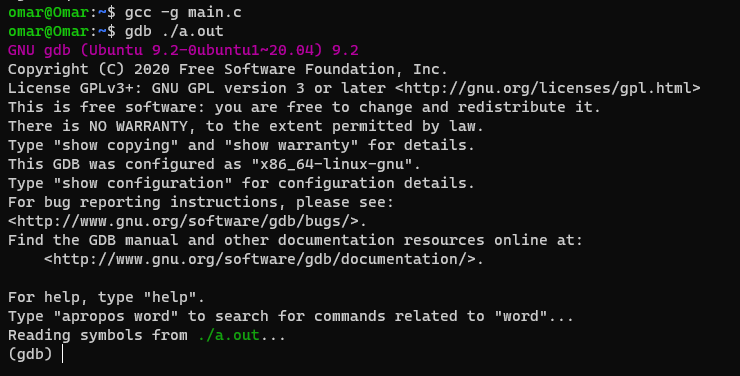
\includegraphics[width=80mm]{resources/loading_gdb}
		\caption{Un programme chargé avec succès par GDB}
	\end{figure}
\end{frame}
	
\begin{frame}{Débogueur: GDB}
	\framesubtitle{Commandes GDB}
	\begin{itemize}
		\item \alert{\texttt{file executable}} : spécifie le programme que vous souhaitez déboguer.
		\item \alert{\texttt{run}} : exécute le programme chargé. des arguments peuvent également être fournis.
		\item \alert{\texttt{list}} : afficher quelques lignes du code source.
		\item \alert{\texttt{break filename:linenumber}} : définit un point d'arrêt sur le numéro de ligne donné dans le fichier source. L'exécution s'arrêtera avant que cette ligne ne soit exécutée.
		\item \alert{\texttt{info breakpoints}} : afficher des informations sur tous les points d'arrêt, y compris son numéro.
		\item \alert{\texttt{delete id}} : supprimer le point d'arrêt numéroté \alert{\texttt{id}}
		\item \alert{\texttt{continue}} : continuera à exécuter le programme à nouveau, après l'avoir arrêté.
	\end{itemize}
\end{frame}

\begin{frame}{Débogueur: GDB}
	\framesubtitle{Commandes GDB}
	\begin{itemize}
		\item \alert{\texttt{info locals}} : Afficher toutes les variables locales
		\item \alert{\texttt{info args}} : Afficher tous les arguments de la fonction en cours d'exécution
		\item \alert{\texttt{backtrace}} : Imprime la pile d'appels jusqu'au point d'arrêt actuel. Utile pour savoir quelles fonctions sont appelées avant qu'un crash ne se produise
		\item \alert{\texttt{backtrace full}} : Comme backtrace mais affiche aussi les variables locales
		\item \alert{\texttt{print expression}} : affichera la valeur de l'expression, qui pourrait être juste un nom de variable.
		\item \alert{\texttt{set varname=value}} : change la valeur d'une variable et continue l'exécution avec la valeur modifiée.
		\item \alert{\texttt{disas}} : affiche le code assembleur de la fonction actuelle.
	\end{itemize}
\end{frame}

\begin{frame}{Débogueur: GDB}
	\framesubtitle{Commandes GDB}
	\begin{itemize}
		\item \alert{\texttt{step}} : exécutera la ligne du code courante, puis arrêtera à nouveau l'exécution avant la ligne suivante.
		\item \alert{\texttt{next}} : est similaire à "step", sauf que si la ligne qui va être exécutée est un appel de fonction, alors cet appel de fonction sera complètement exécuté avant que l'exécution ne s'arrête à nouveau.
		\item \alert{\texttt{until}} : comme \alert{\texttt{next}}, sauf que si vous êtes à la fin d'une boucle, \alert{\texttt{until}} continuera l'exécution jusqu'à ce que la fin de la boucle. Ceci est pratique si vous voulez voir ce qui se passe après une boucle, mais que vous ne voulez pas parcourir chaque itération.
		\item \alert{\texttt{finish}} : continuer l'exécution jusqu'à la fin de la fonction courante.
		\item \alert{\texttt{where}} : affiche le numéro de ligne en cours d'exécution
	\end{itemize}
\end{frame}

\subsection{Valgrind}
\begin{frame}{Détecter les fuites : Valgrind}
	\begin{block}{Qu'est-ce que Valgrind?}
		Valgrind est un outil de programmation pour le débogage de la mémoire, la détection des fuites de mémoire et le profilage.
	\end{block}
	\begin{alertblock}{Attention : }
		\begin{itemize}
			\item Comme pour GDB, pour que valgrind fonctionne correctement, votre programme doit être compilé avec l'option \alert{\texttt{-g}}.
			\item valgrind n'est pas installé par défaut. Vous devez l'installer manuellement.
		\end{itemize}
	\end{alertblock}
\end{frame}

\begin{frame}{Détecter les fuites : Valgrind}
	\framesubtitle{Guide d'utilisation}
	\begin{block}{Comment l'utiliser ?}
		Une fois que vous avez compilé votre programme dans les bonnes configurations. Utiliser Valgrind est simple. Il suffit d'utiliser la commande suivante : \\ 
		\alert{\texttt{valgrind -{}-leak-check=yes nom\_programme [[ args ]]}} \\
		Les arguments \texttt{[[ args ]]} sont facultatifs, mais si votre programme en a besoin, vous pouvez les transmettre de la manière mentionnée ci-dessus.
	\end{block}
\end{frame}

\defverbatim[colored]\valgrindExmpl{	
\begin{lstlisting}[language=C,tabsize=4]
#include <stdlib.h>
	
void toto()
{
	int* x = malloc(5 * sizeof(int));
	x[6] = 0;
}
	
int main()
{
	toto();
}
\end{lstlisting}}
\begin{frame}{Détecter les fuites : Valgrind}
	\framesubtitle{Guide d'utilisation : Exemple}
	Soit le code suivant :
	\valgrindExmpl
\end{frame}

\defverbatim[colored]\valgrindExmplSolution{	
\begin{lstlisting}[language=C,tabsize=4]
#include <stdlib.h>

void toto()
{
	int* tab = malloc(5 * sizeof(int));
	tab[6] = 0; // problem 1 : Exceeding allocated memory 
				// boundaries
			    // problem 2 : memory leak, tab is not freed
}

int main()
{
	toto();
}
\end{lstlisting}}
\begin{frame}{Détecter les fuites : Valgrind}
	\framesubtitle{Guide d'utilisation : Exemple}
	Compilation avec la commande : \texttt{gcc -g main.c} \\
	Execution du valgrind avec la commande :\\
	\texttt{valgrind -{}-leak-check=yes ./a.out}
	\begin{figure}[!h]
		\centering
		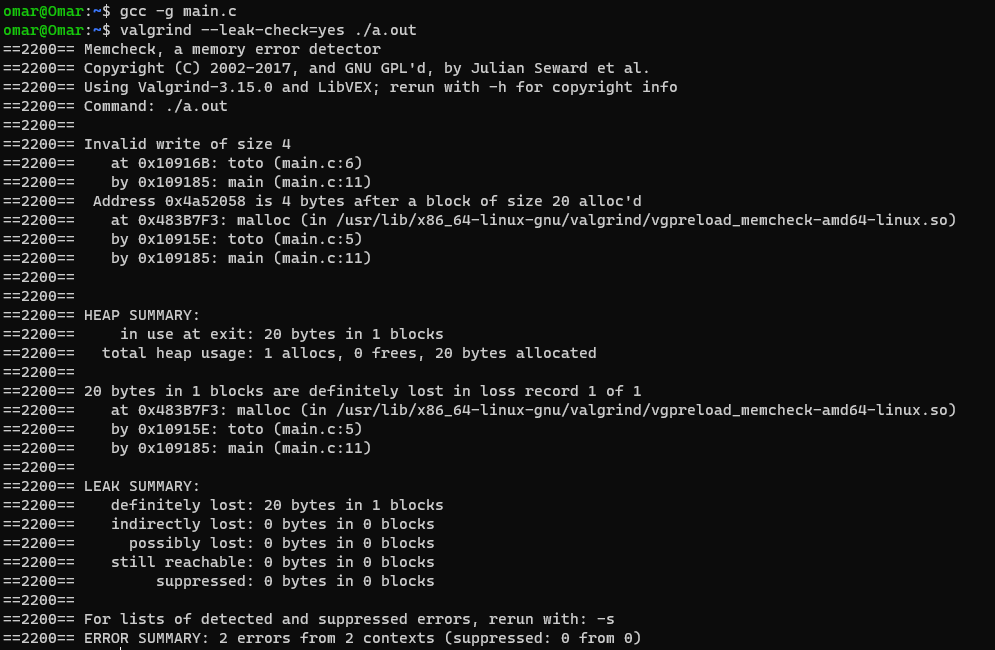
\includegraphics[width=77mm]{resources/valgrind}
		\caption{La sortie Valgrind lors de l'exécution}
	\end{figure}
\end{frame}

\defverbatim[colored]\valgrindOutputOne{	
\begin{lstlisting}[language=C,tabsize=4]
==2200== Invalid write of size 4
==2200==    at 0x10916B: toto (main.c:6)
==2200==    by 0x109185: main (main.c:11)
==2200==  Address 0x.. is 4 bytes after a block of size 20 allocd
==2200==    at 0x483B7F3: malloc (vgpreload_memcheck.so)
==2200==    by 0x10915E: toto (main.c:5)
==2200==    by 0x109185: main (main.c:11)
\end{lstlisting}}
\begin{frame}{Détecter les fuites : Valgrind}
	\framesubtitle{Comment interpréter le résultat}
	\valgrindOutputOne
\end{frame}


\begin{frame}{Détecter les fuites : Valgrind}
	\framesubtitle{Comment interpréter le résultat}
	\begin{block}{Explication : }
		- Le numéro \texttt{2200} est le PID du processus, c'est n'est pas trés important pour nous.\\
		- \alert{Ligne 1} : indique une écriture de 4 octets dans une zone mémoire qui n'appartient pas au processus. Ce qui est affiché après est la pile d'appels menant à cette erreur. \\
		- \alert{Ligne 4} : donne plus détail sur l'erreur à la ligne 1. il précise l'adresse où l'écriture s'est produite et la position de cette adresse par rapport à ce que nous avons alloué auparavant. Il montre également d'où provient cette adresse en affichant la pile d'appels.
	\end{block}
\end{frame}


\defverbatim[colored]\valgrindOutputTwo{	
\begin{lstlisting}[language=C,tabsize=4]
20 bytes in 1 blocks are definitely lost in loss record 1 of 1
   at 0x483B7F3: malloc (in vgpreload_memcheck.so)
   by 0x10915E: toto (main.c:5)
   by 0x109185: main (main.c:11)
\end{lstlisting}}
\begin{frame}{Détecter les fuites : Valgrind}
	\framesubtitle{Comment interpréter le résultat}
	\valgrindOutputTwo
	\begin{block}{Explication : }
		- \alert{Ligne 1} : indique qu'il y a un fuite de mémoire de \texttt{20} octets qui sont définitivement perdu. Les lignes juste après montrent la pile d'appels qui indique où la mémoire perdu a été allouée. \\
		- Malheureusement, Valgrind ne peut pas vous dire \alert{pourquoi} la mémoire a fui.
	\end{block}
\end{frame}

\begin{frame}{Détecter les fuites : Valgrind}
	\begin{alertblock}{ATTENTION : }
		- En fait, valgrind étant un framework, il peut faire plus que simplement détecter les fuites. Il fournit une suite d'outils et les outils que nous utilisons jusqu'à présent s'appellent \alert{Memcheck}. \\
		- \alert{Memcheck} n'est pas parfait; il produit parfois de faux positifs, et il existe des mécanismes pour supprimer ces effets secondaires. Cependant, il est généralement correct 99\% du temps, vous devez donc éviter \alert{d'ignorer} ses messages d'erreur.\\
		- \alert{Memcheck} ne peut pas détecter toutes les erreurs de mémoire. Par exemple, il ne peut pas détecter les lectures ou écritures hors limites dans des tableaux alloués statiquement sur la pile. Mais il devrait détecter de nombreuses erreurs qui pourraient planter le programme (par exemple, les erreurs de segmentation).
	\end{alertblock}
\end{frame}

\begin{frame}{Valgrind}
	\framesubtitle{Détecter la mémoire non initialisée}
	\begin{block}{Que peut-il faire d'autre pour nous?}
		Valgrind signale également les utilisations de valeurs \alert{non initialisées}, le plus souvent avec le message "Le saut ou le déplacement conditionnel dépend de la ou des valeurs non initialisées". \\
		Il peut être difficile de déterminer la cause de ces erreurs. Essayez d'utiliser \alert{\texttt{-{}-track-origins=yes}} pour obtenir des informations supplémentaires.
	\end{block}
\end{frame}

\begin{frame}{Valgrind}
	\framesubtitle{Valgrind : Au-delà de la vérification de la mémoire}
	Comme mentionné précédemment, Valgrind peut fournir un ensemble de services qui sortent du cadre de ce cours, nous ne les couvrirons donc pas ici. Parmi ces outils, on retrouve :
	\begin{itemize}
		\item \alert{\texttt{Massif}} : un profileur de tas, mesure l'utilisation de la mémoire du tas au fil du temps.
		\item \alert{\texttt{Cachegrind}} : un profileur de cache, mesurer les succès et les échecs du cache et éventuellement les prédictions de branche.
		\item \alert{\texttt{Callgrind}} : outil de profilage qui enregistre l'historique des appels des fonctions d'un programme sous forme d'un graphe.
		\item \alert{\texttt{Helgrind }} : détecte les conditions de concurrence dans le code multithread.
	\end{itemize}
\end{frame}

  	
  	\begin{frame}{Conclusion}
  		\framesubtitle{Les dix commandements pour réussir en C}
  		\begin{itemize}
  			\item 1.	
  			\item 2.	
  			\item 3.	
  			\item 4.	
  			\item 5.
  			\item 6.	
  			\item 7.	
  			\item 8.	
  			\item 9.	
  			\item 10.	
  		\end{itemize}
  	\end{frame}
  \end{darkframes}
\end{document}
